\documentclass[research]{BMSTU-IU8}

\usepackage{fontspec}
\setmainfont{Times New Roman}
\setromanfont{Times New Roman}
\setsansfont{Arial}
\setmonofont{Courier New}

\usepackage{amsmath}
\usepackage{amssymb}
\usepackage{subcaption}
\usepackage{todonotes}
\usepackage{lipsum}
\usepackage{tikz}
\usepackage{pgfplots}

\student{Санджиев Т. С.}
\theme{Классификатор адресов в сети криптовалюты Bitcoin}
\group{ИУ8-93-2024}

\studentFullName{Санджиев Темирхан Санджиевич}
\profile{20У951}
\speciality{10.05.03 <<Информационная безопасность автоматизированных систем>>}
\specialization{10.05.03\_03 <<Создание автоматизированных систем в защищенном исполнении>>}
\supervisorWithDegree{профессор кафедры ИУ8 Зуев Юрий Анатольевич}
\supervisor{Зуев Ю. А.}

\addbibresource{main.bib}
% Сокращения и обозначения
\newacronym{adasyn}{ADASYN}{Adaptive Synthetic Sampling}
\newacronym{aml}{AML}{Anti-Money Laundering}
\newacronym{api}{API}{Application Programming Interface}
\newacronym{auc}{AUC}{Area Under the Curve}
\newacronym{btc}{BTC}{Bitcoin}
\newacronym{cpu}{CPU}{Central Processing Unit}
\newacronym{csv}{CSV}{Comma-Separated Values}
\newacronym{dl}{DL}{Deep Learning}
\newacronym{f1}{F1}{F1-мера}
\newacronym{gat}{GAT}{Graph Attention Network}
\newacronym{gcn}{GCN}{Graph Convolutional Network}
\newacronym{gnn}{GNN}{Graph Neural Network}
\newacronym{gpu}{GPU}{Graphics Processing Unit}
\newacronym{json}{JSON}{JavaScript Object Notation}
\newacronym{kyc}{KYC}{Know Your Customer}
\newacronym{ln}{LN}{Lightning Network}
\newacronym{lstm}{LSTM}{Long Short-Term Memory}
\newacronym{ml}{ML}{Machine Learning}
\newacronym{mlp}{MLP}{Multilayer Perceptron}
\newacronym{nn}{NN}{Neural Network}
\newacronym{pca}{PCA}{Principal Component Analysis}
\newacronym{pow}{PoW}{Proof of Work}
\newacronym{ram}{RAM}{Random Access Memory}
\newacronym{relu}{ReLU}{Rectified Linear Unit}
\newacronym{roc}{ROC}{Receiver Operating Characteristic}
\newacronym{segwit}{SegWit}{Segregated Witness}
\newacronym{shap}{SHAP}{SHapley Additive exPlanations}
\newacronym{smote}{SMOTE}{Synthetic Minority Over-sampling Technique}
\newacronym{txid}{TXID}{Transaction Identifier}
\newacronym{utxo}{UTXO}{Unspent Transaction Output}

% Термины и определения
\newglossaryentry{id4}{
    name={Адрес},
    description={Уникальный идентификатор в сети Bitcoin, используемый для отправки и получения средств}
}

\newglossaryentry{id15}{
    name={Батч},
    description={Подмножество обучающих данных, используемое для одного шага обновления весов нейронной сети}
}

\newglossaryentry{id2}{
    name={Блокчейн},
    description={Распределённая база данных, состоящая из последовательно связанных блоков, содержащих информацию о транзакциях}
}

\newglossaryentry{id10}{
    name={Гиперпараметр},
    description={Параметр модели или процесса обучения, задаваемый до начала обучения и не изменяемый в его ходе}
}

\newglossaryentry{id20}{
    name={Граф транзакций},
    description={Графовое представление Bitcoin-сети, где узлами являются адреса, а рёбрами~--- транзакции между ними}
}

\newglossaryentry{id7}{
    name={Датасет},
    description={Набор данных, используемый для обучения, тестирования и валидации алгоритмов машинного обучения}
}

\newglossaryentry{id14}{
    name={Дропаут},
    description={Метод регуляризации нейронных сетей, при котором случайные нейроны отключаются во время обучения для предотвращения переобучения}
}

\newglossaryentry{id19}{
    name={Извлечение признаков},
    description={Процесс выделения характеристик из данных для использования в алгоритмах машинного обучения}
}

\newglossaryentry{id13}{
    name={Классификация},
    description={Задача машинного обучения, заключающаяся в отнесении объектов к предопределённым классам}
}

\newglossaryentry{id11}{
    name={Кросс-валидация},
    description={Метод оценки качества модели путём разбиения данных на несколько частей и поочерёдного использования каждой из них в качестве тестовой}
}

\newglossaryentry{id12}{
    name={Матрица ошибок},
    description={Таблица, отображающая соотношение предсказанных и истинных классов, используемая для оценки качества классификации}
}

\newglossaryentry{id6}{
    name={Нейронная сеть},
    description={Вычислительная модель, вдохновлённая биологическими нейронными сетями, состоящая из слоёв взаимосвязанных узлов, обучаемых на данных}
}

\newglossaryentry{id8}{
    name={Обучение модели},
    description={Процесс настройки параметров нейронной сети путём минимизации функции потерь на обучающей выборке}
}

\newglossaryentry{id18}{
    name={Оптимизатор},
    description={Алгоритм, обновляющий параметры модели на основе вычисленных градиентов с целью минимизации функции потерь}
}

\newglossaryentry{id9}{
    name={Переобучение},
    description={Явление, при котором модель слишком точно подстраивается под обучающую выборку и теряет способность к обобщению}
}

\newglossaryentry{id3}{
    name={Транзакция},
    description={Операция передачи Bitcoin между адресами, записанная в блокчейне}
}

\newglossaryentry{id17}{
    name={Функция потерь},
    description={Функция, измеряющая расхождение между предсказаниями модели и истинными метками, минимизируемая в процессе обучения}
}

\newglossaryentry{id16}{
    name={Эпоха},
    description={Один полный проход по всему обучающему датасету в ходе обучения нейронной сети}
}

\newglossaryentry{id1}{
    name={Bitcoin},
    description={Криптовалюта и одноимённая платёжная система, использующая технологию блокчейн для децентрализованного учёта транзакций}
}

\newglossaryentry{id5}{
    name={UTXO},
    description={Unspent Transaction Output~--- модель учёта средств в Bitcoin, где каждый выход транзакции может быть потрачен только один раз}
}


\begin{document}
    \maketitle

    \setcounter{page}{4}

    \abstract % Структурный элемент: РЕФЕРАТ
В рамках работы разработан и апробирован программный комплекс для классификации Bitcoin-адресов по типу кошелька на основе датасета, сформированного в ходе предшествующих НИРС. Реализован полный пайплайн обработки данных: удаление высококоррелированных признаков, автоматический выбор стратегии устранения дисбаланса классов (SMOTE против ADASYN), стандартизация. Обучено шесть моделей машинного обучения: MLP, Random Forest, XGBoost, LightGBM, Stacking и kNN. Для деревьевидных моделей выполнена настройка гиперпараметров методом случайного поиска с кросс-валидацией. Проведена комплексная оценка качества: построены матрицы ошибок, ROC-кривые, вычислены взвешенная F1-мера и макро-усреднённый ROC-AUC. Для лучшей модели выполнена оптимизация порогов классификации по критерию Юдена и интерпретация предсказаний методом SHAP. Наилучший результат достигнут моделью XGBoost: взвешенная F1-мера~--- 0,7907; ROC-AUC~--- 0,9610.

Ключевые слова: Bitcoin, блокчейн, классификация адресов, машинное обучение, XGBoost, LightGBM, нейронная сеть, Stacking, SMOTE, SHAP.


    \tableofcontents
    \termsanddefenitions
    \listofabbreviations

    \introduction % Структурный элемент: ВВЕДЕНИЕ

Криптовалюта Bitcoin, созданная в 2008 году Сатоши Накамото~\cite{bitcoin_whitepaper}, продолжает оставаться наиболее капитализированной и широко используемой децентрализованной платёжной системой. В её основе лежит технология распределённого реестра~--- блокчейна~--- представляющего собой публично доступную цепочку блоков транзакций, подтверждённых майнерами посредством алгоритма~\acrshort{pow}. Публичная природа блокчейна обеспечивает полную верифицируемость транзакций, однако участники сети идентифицируются лишь псевдонимными адресами~--- хешами открытых ключей~--- без привязки к реальным личностям. Это создаёт серьёзные вызовы для регуляторов, правоохранительных органов и аналитиков финансовых рисков, заинтересованных в выявлении подозрительной активности: отмывания денег, мошенничества, финансирования незаконной деятельности.

Классификация Bitcoin-адресов по типу деятельности~--- задача, решение которой позволяет частично снять псевдоанонимность участников сети. Если известно, что некоторый адрес принадлежит бирже или майнинговому пулу, аналитик может интерпретировать транзакции с этим адресом и реконструировать финансовые потоки. В отличие от ручного анализа или эвристических методов, основанных на фиксированных правилах, подходы на основе машинного обучения позволяют автоматически выявлять сложные паттерны в пространстве признаков, масштабироваться на большие объёмы данных и адаптироваться к новым видам активности.

В ходе предшествующих научно-исследовательских работ~(НИРС-01 и НИРС-02) были решены задачи систематизации существующих алгоритмов классификации транзакций, сбора Bitcoin-адресов из открытых источников, извлечения 34 транзакционных признаков через~\acrshort{api} Bitcoin-эксплорера и формирования датасета объёмом 8\,115 адресов с разметкой по шести типам кошельков. Выявлена существенная несбалансированность классов~(коэффициент~$\approx$~39,85) и определён набор наиболее информативных признаков.

Настоящая работа является третьим этапом исследовательского цикла и посвящена практическому применению подготовленного датасета: обучению, настройке гиперпараметров и сравнительной оценке моделей классификации Bitcoin-адресов, а также интерпретации полученных результатов.

Актуальность работы обусловлена:
\begin{itemize}
    \item ростом объёма криптовалютных транзакций и потребностью в масштабируемых автоматизированных инструментах мониторинга~--- ручной анализ блокчейна в современных масштабах практически невозможен;
    \item регуляторными требованиями соблюдения процедур \acrshort{aml}/\acrshort{kyc} в криптовалютной сфере, которые обязывают биржи и сервисы идентифицировать контрагентов;
    \item научным интересом к применению ансамблевых методов машинного обучения для анализа высокодимензиональных блокчейн-данных с дисбалансом классов;
    \item необходимостью сравнительного анализа нейросетевых и деревьевидных подходов на табличных Bitcoin-данных.
\end{itemize}

Целью данной научно-исследовательской работы является разработка, обучение и сравнительная оценка ансамблевых и нейросетевых моделей классификации Bitcoin-адресов по типам кошельков на основе датасета, подготовленного в предшествующих НИРС, а также анализ качества и интерпретируемости полученных результатов.

Для достижения цели поставлены следующие задачи:
\begin{itemize}
    \item Подготовка признакового пространства: удаление высококоррелированных признаков, выбор и применение стратегии устранения дисбаланса классов, стандартизация данных;
    \item Обучение шести моделей машинного обучения: MLP, Random Forest, XGBoost, LightGBM, Stacking и kNN;
    \item Настройка гиперпараметров деревьевидных моделей методом случайного поиска с кросс-валидацией;
    \item Оценка качества обученных моделей с использованием метрик взвешенной F1-меры и макро-усреднённого ROC-AUC на отложенной тестовой выборке;
    \item Оптимизация порогов классификации лучшей модели по критерию Юдена~--- для улучшения полноты на миноритарных классах;
    \item Интерпретация предсказаний лучшей модели методом~\acrshort{shap} для выявления наиболее значимых признаков;
    \item Сравнительный анализ всех обученных моделей и формулировка рекомендаций по дальнейшему улучшению.
\end{itemize}


    \section{Обучение моделей классификации на данных, полученных в предыдущих НИРС}

\subsection{Подготовка данных к обучению}

Исходным материалом для данного этапа служит датасет, сформированный в рамках НИРС-02~\cite{github_repo_nirs2}. Датасет содержит 8\,115 Bitcoin-адресов, каждый из которых описывается 34 признаками. Признаки сгруппированы по смыслу:
\begin{itemize}
    \item \textit{структурные}~--- число входов и выходов транзакций, количество уникальных контрагентов, средняя вентиляторность (fan-in/fan-out);
    \item \textit{UTXO-паттерны}~--- доля нераспределённых выходов, средний остаток на адресе, характеристики типичного изменения UTXO;
    \item \textit{временны́е}~--- общий период активности адреса, средний интервал между транзакциями, число активных дней;
    \item \textit{экономические}~--- суммарный объём входящих и исходящих средств (в satoshi), средний объём одной транзакции, соотношение объёмов;
    \item \textit{Bitcoin-специфичные}~--- наличие SegWit-выходов, участие в мультиподписных схемах, паттерны округления сумм.
\end{itemize}

Целевая переменная~--- тип кошелька~--- принимает шесть значений: майнеры~(\textit{miner},~3\,547 адресов, 43,7\%), биржи~(\textit{exchange},~1\,532, 18,9\%), сервисы~(\textit{services},~1\,249, 15,4\%), азартные игры~(\textit{gambling},~911, 11,2\%), операции типа CoinJoin~(\textit{coinjoin-like},~787, 9,7\%) и майнинговые пулы~(\textit{mining\_pool},~89, 1,1\%).

\subsubsection{Отбор признаков и устранение мультиколлинеарности}

Наличие высококоррелированных признаков в обучающей выборке нежелательно: оно не несёт дополнительной информации, но увеличивает размерность пространства, замедляет обучение и может нестабилизировать оценки важности признаков. Степень линейной зависимости между парой непрерывных признаков $x_i$, $x_j$ измеряется коэффициентом корреляции Пирсона:
\[
    r(x_i, x_j) = \frac{\sum_{k=1}^{n}(x_i^{(k)} - \bar{x}_i)(x_j^{(k)} - \bar{x}_j)}
    {\sqrt{\sum_{k=1}^{n}(x_i^{(k)} - \bar{x}_i)^2 \cdot \sum_{k=1}^{n}(x_j^{(k)} - \bar{x}_j)^2}},
\]
где $x_i^{(k)}$, $x_j^{(k)}$~--- значения признаков $x_i$ и $x_j$ для $k$-го образца; $\bar{x}_i$, $\bar{x}_j$~--- их выборочные средние; $n$~--- число образцов. Если $|r(x_i, x_j)| > 0{,}95$, один из признаков удаляется. По результатам автоматического анализа корреляционной матрицы исключены четыре признака: \textit{unique\_input\_addresses} и \textit{unique\_output\_addresses}~--- как практически линейно зависимые от агрегированных счётчиков входов и выходов,~--- а также два дополнительных признака, выявленных алгоритмом попарной проверки. Итоговое признаковое пространство составляет~30 переменных.

\subsubsection{Разбиение выборки}

Датасет разбивается на три непересекающихся подмножества: обучающую выборку~(70\%), валидационную~(15\%) и тестовую~(15\%). Разбиение выполняется стратифицированно~--- пропорции классов сохраняются во всех трёх частях. Это критически важно при дисбалансе: нестратифицированное разбиение может случайно недопредставить миноритарный класс~(\textit{mining\_pool},~89 образцов) в тестовой выборке, что сделает оценку качества нестабильной. После стратификации в тестовой выборке находится~$\lceil 89 \cdot 0{,}15 \rceil = 14$~адресов класса~\textit{mining\_pool}.

Важно, что оверсэмплинг и нормализация применяются исключительно к обучающей выборке, тогда как валидационная и тестовая выборки остаются в исходном виде~--- это исключает утечку данных (data leakage) и обеспечивает объективную оценку обобщающей способности модели.

\subsubsection{Устранение дисбаланса классов}

Дисбаланс классов с коэффициентом $\approx$~39,85 (отношение числа образцов мажоритарного класса к миноритарному) является существенной проблемой: классификатор, обученный на несбалансированных данных, стремится максимизировать суммарную точность за счёт занижения предсказаний для редких классов. Для устранения дисбаланса рассматриваются два метода оверсэмплинга:

\textbf{SMOTE}~(\acrlong{smote})~\cite{smote_paper}~--- для каждого образца миноритарного класса $\mathbf{x}_i$ выбирается $k$ ближайших соседей того же класса~(по умолчанию $k=5$). Синтетический образец $\tilde{\mathbf{x}}$ формируется интерполяцией:
\[
    \tilde{\mathbf{x}} = \mathbf{x}_i + \lambda \cdot (\mathbf{x}_{nn} - \mathbf{x}_i), \quad \lambda \sim U(0, 1),
\]
где $\tilde{\mathbf{x}}$~--- синтетический образец; $\mathbf{x}_i$~--- исходный образец миноритарного класса; $\mathbf{x}_{nn}$~--- случайно выбранный из $k$ ближайших соседей образец того же класса; $\lambda \sim U(0,1)$~--- коэффициент интерполяции. Такой подход создаёт разнообразные, но не выходящие за пределы выпуклой оболочки класса образцы.

\textbf{ADASYN}~(\acrlong{adasyn})~--- адаптивная модификация SMOTE, при которой интенсивность генерации для каждого образца пропорциональна плотности ошибок в его окрестности: больше синтетических примеров генерируется там, где класс труднее всего отделить от мажоритарных. Формально для образца $\mathbf{x}_i$ вычисляется $r_i = \Delta_i / K$, где $\Delta_i$~--- число соседей из мажоритарного класса среди $K$ ближайших соседей образца $\mathbf{x}_i$~--- доля таких соседей; число синтетических образцов для $\mathbf{x}_i$ пропорционально $\hat{r}_i = r_i / \sum_j r_j$, где суммирование ведётся по всем образцам миноритарного класса.

Выбор между SMOTE и ADASYN производится автоматически: прокси-модель Random Forest~(50 деревьев) обучается раздельно на каждом варианте оверсэмплинга и оценивается по взвешенной F1-мере на оригинальной~(не синтетической) валидационной выборке. По результатам сравнения выбран SMOTE~(val~F1~=~0,7475 против 0,7337 у ADASYN). Предпочтение SMOTE объясняется тем, что ADASYN, концентрируя генерацию в граничных зонах, увеличивает шум в разделяющей гиперплоскости~--- это может ухудшать обобщение. После применения SMOTE обучающая выборка расширяется до~14\,892~образцов с равным представлением каждого класса.

Дополнительно модели Random Forest и LightGBM обучаются с параметром \texttt{class\_weight="balanced"}, который масштабирует веса ошибок обратно пропорционально частоте класса. Это приводит к тому, что ошибка на одном образце класса \textit{mining\_pool} штрафуется примерно в 40 раз сильнее, чем ошибка на образце класса \textit{miner}.

\subsubsection{Стандартизация признаков}

После оверсэмплинга признаки стандартизируются методом \textit{StandardScaler}: каждый признак $x_j$ преобразуется к нулевому среднему и единичному стандартному отклонению:
\[
    \hat{x}_j = \frac{x_j - \mu_j}{\sigma_j},
\]
где $x_j$~--- исходное значение $j$-го признака; $\hat{x}_j$~--- его стандартизованное значение; $\mu_j$ и $\sigma_j$~--- среднее и стандартное отклонение признака $j$, вычисленные по обучающей выборке~\cite{scikit_learn}. Стандартизация необходима для MLP и kNN, поскольку оба метода чувствительны к масштабу признаков; для деревьевидных методов она не влияет на результат, однако сохраняется для унификации пайплайна.

\subsection{Обучение MLP}

Полносвязная нейронная сеть~(\acrshort{mlp}) рассматривается как основная нейросетевая модель в данной работе. MLP~--- это направленный граф слоёв нейронов: входной слой принимает вектор стандартизованных признаков размерности~30; далее следуют три скрытых слоя~(256, 128 и 64 нейрона); выходной слой содержит 6 нейронов~--- по одному на класс~--- с функцией активации~\textit{Softmax}, преобразующей логиты в вектор вероятностей.

На каждом скрытом слое применяется функция активации~\acrshort{relu}:
\[
    \text{ReLU}(z) = \max(0, z),
\]
где $z$~--- взвешенная сумма входов нейрона. Функция обеспечивает нелинейность преобразования и устраняет проблему затухающих градиентов. Обучение производится методом обратного распространения ошибки: вычисляется градиент функции потерь по всем весам сети, после чего веса обновляются оптимизатором Adam~\cite{adam_optimizer}~--- адаптивным стохастическим градиентным спуском с моментом первого и второго порядка:
\[
    \theta_{t+1} = \theta_t - \frac{\eta}{\sqrt{\hat{v}_t} + \varepsilon} \cdot \hat{m}_t,
\]
где $\theta_t$~--- вектор параметров модели на шаге $t$; $\hat{m}_t$ и $\hat{v}_t$~--- скорректированные на смещение оценки первого и второго момента градиента; $\eta$~--- скорость обучения; $\varepsilon$~--- малая константа для численной стабильности. В качестве функции потерь используется кросс-энтропия.

Для предотвращения переобучения применяется L2-регуляризация~(\textit{weight decay}) с коэффициентом~$\alpha = 10^{-4}$: к функции потерь добавляется штрафной член $\alpha \|\mathbf{W}\|_F^2$, препятствующий росту весов. Дополнительно используется ранняя остановка (\textit{early stopping}): если взвешенная F1-мера на валидационной доле обучающей выборки~(10\%) не улучшается на протяжении 10~итераций подряд, обучение прекращается и восстанавливаются веса с наилучшим значением метрики.

Гиперпараметры MLP зафиксированы по результатам предварительных экспериментов без использования автоматического поиска: объём обучающей выборки~(14\,892~образцов) в сочетании с высокой сложностью MLP делает перебор конфигураций через кросс-валидацию нецелесообразным по времени. Итоговые параметры: скорость обучения~$5 \cdot 10^{-4}$, размер батча~32, $\alpha = 10^{-4}$, максимальное число итераций~200.

\subsection{Ансамблевые методы}

\subsubsection{Random Forest}

Random Forest~\cite{scikit_learn}~--- ансамблевый метод, основанный на принципе бэггинга~(\textit{bootstrap aggregating}): для каждого из $B$ деревьев формируется бутстрэп-подвыборка~(с возвращением) из обучающей выборки, а при выборе оптимального разбиения в каждом узле рассматривается случайное подмножество признаков размером~$\sqrt{p}$ или~$\log_2 p$. Итоговый класс определяется мажоритарным голосованием деревьев. Случайность при отборе признаков снижает корреляцию между деревьями и повышает устойчивость ансамбля к переобучению.

Для борьбы с дисбалансом классов используется параметр \texttt{class\_weight="balanced"}, при котором вес каждого класса $c$ задаётся как $w_c = n / (K \cdot n_c)$, где $n$~--- полное число образцов, $K$~--- число классов, $n_c$~--- число образцов класса $c$.

Пространство поиска гиперпараметров:
\begin{itemize}
    \item число деревьев $B$: $\{100, 200\}$;
    \item максимальная глубина дерева: $\{\text{без ограничения},\; 15\}$;
    \item минимальное число образцов для разбиения узла: $\{2,\; 5\}$;
    \item число признаков при разбиении: $\{\sqrt{p},\; \log_2 p\}$.
\end{itemize}

\subsubsection{XGBoost}

XGBoost~\cite{xgboost_paper}~--- реализация градиентного бустинга на деревьях решений. В отличие от бэггинга, бустинг строит деревья последовательно: каждое новое дерево $h_t$ обучается аппроксимировать отрицательный градиент функции потерь $\mathcal{L}$ по предсказаниям текущего ансамбля. Итоговый ансамбль~--- аддитивная модель:
\[
    F_T(\mathbf{x}) = \sum_{t=1}^{T} \eta \cdot h_t(\mathbf{x}),
\]
где $F_T(\mathbf{x})$~--- итоговое предсказание ансамбля из $T$ деревьев для объекта $\mathbf{x}$; $h_t(\mathbf{x})$~--- предсказание $t$-го дерева; $\eta$~--- скорость обучения, масштабирующая вклад каждого дерева.

Ключевое отличие XGBoost~--- включение в целевую функцию регуляризационных членов, штрафующих сложность каждого дерева:
\[
    \widetilde{\mathcal{L}}^{(t)} = \sum_{i} l\bigl(y_i,\, \hat{y}_i^{(t)}\bigr) + \gamma T_t + \frac{1}{2}\lambda \|\mathbf{w}_t\|^2,
\]
где $\widetilde{\mathcal{L}}^{(t)}$~--- регуляризованная целевая функция на шаге $t$; $l(y_i, \hat{y}_i^{(t)})$~--- функция потерь для $i$-го обучающего образца; $y_i$~--- истинная метка класса; $\hat{y}_i^{(t)}$~--- текущее предсказание ансамбля; $T_t$~--- число листьев добавляемого дерева; $\mathbf{w}_t$~--- вектор весов листьев; $\gamma$ и $\lambda$~--- гиперпараметры регуляризации. Это предотвращает переобучение даже на глубоких деревьях.

Пространство поиска гиперпараметров:
\begin{itemize}
    \item число деревьев $T$: $\{100, 200\}$;
    \item максимальная глубина дерева: $\{4,\; 6\}$;
    \item скорость обучения $\eta$: $\{0{,}1;\; 0{,}2\}$;
    \item доля случайно выбираемых образцов для дерева~(\textit{subsample}): $\{0{,}8;\; 1{,}0\}$;
    \item доля случайно выбираемых признаков~(\textit{colsample\_bytree}): $\{0{,}8;\; 1{,}0\}$.
\end{itemize}

Параметры \textit{subsample} и \textit{colsample\_bytree} вносят стохастичность, аналогичную бэггингу, и снижают корреляцию между деревьями.

\subsubsection{LightGBM}

LightGBM~\cite{lightgbm_paper}~--- высокопроизводительная реализация градиентного бустинга, использующая два ключевых нововведения. Во-первых, \textit{алгоритм листового роста}: вместо уровневого (depth-wise) наращивания дерева LightGBM на каждом шаге добавляет лист к узлу с наибольшим приростом функции. Это позволяет строить глубокие несимметричные деревья за меньшее число шагов. Во-вторых, \textit{гистограммная аппроксимация}: непрерывные признаки дискретизируются в $B$ бинов~(по умолчанию 255), что снижает вычислительную сложность поиска оптимального разбиения с $O(n \cdot p)$ до $O(B \cdot p)$. В совокупности это обеспечивает скорость обучения в 10--100 раз выше, чем у XGBoost, при сопоставимом качестве.

Используется параметр \texttt{class\_weight="balanced"}. Пространство поиска:
\begin{itemize}
    \item число деревьев: $\{100, 200\}$;
    \item максимальная глубина дерева: $\{4,\; 6,\; -1\}$~(без ограничения);
    \item скорость обучения: $\{0{,}1;\; 0{,}2\}$;
    \item максимальное число листьев~(\textit{num\_leaves}): $\{31,\; 63\}$;
    \item доля образцов для построения дерева~(\textit{subsample}): $\{0{,}8;\; 1{,}0\}$.
\end{itemize}

Параметр \textit{num\_leaves} является основным регулятором сложности в LightGBM: при листовом росте глубина дерева сама по себе не ограничивает сложность, поэтому ограничение числа листьев эквивалентно ограничению глубины в XGBoost.

\subsubsection{Stacking}

Stacking~(\textit{StackingClassifier})~--- двухуровневый ансамбль. На первом уровне три базовых модели~--- Random Forest, XGBoost и LightGBM~--- обучаются на обучающей выборке. Для формирования признаков мета-уровня применяется трёхкратная стратифицированная кросс-валидация: обучающая выборка делится на три фолда; каждая базовая модель обучается на двух фолдах и предсказывает вероятности для третьего. Таким образом для каждого объекта обучающей выборки вычисляется вектор вероятностей без использования самого объекта в обучении~--- это исключает утечку данных. Итоговая матрица мета-признаков имеет размерность $n_{\text{train}} \times (3 \cdot K)$, где~$K = 6$~--- число классов.

На втором уровне мета-классификатор~--- логистическая регрессия~--- обучается на мета-признаках. При оценке на тестовой выборке базовые модели дообучаются на полной обучающей выборке и формируют мета-признаки для тестовых объектов; затем мета-классификатор выдаёт финальное предсказание.

\subsubsection{kNN}

kNN~--- непараметрический классификатор, не требующий явного обучения. Для классификации нового объекта $\mathbf{x}_{\text{test}}$ вычисляется евклидово расстояние до всех объектов обучающей выборки, отбираются $k$ ближайших, и класс определяется большинством голосов:
\[
    \hat{y} = \arg\max_{c} \sum_{i \in N_k(\mathbf{x}_{\text{test}})} \mathbf{1}[y_i = c],
\]
где $\hat{y}$~--- предсказанный класс; $c$~--- перебираемый класс; $N_k(\mathbf{x}_{\text{test}})$~--- множество индексов $k$ ближайших соседей объекта $\mathbf{x}_{\text{test}}$; $y_i$~--- истинная метка $i$-го соседа; $\mathbf{1}[\cdot]$~--- индикаторная функция. Используется $k=7$ без дополнительной настройки~--- как простейший базовый классификатор. Метод чувствителен к масштабу признаков~(поэтому необходима стандартизация) и к «проклятию размерности» в высокодимензиональных пространствах, однако хорошо иллюстрирует, насколько линейно не разделимы классы в исходном признаковом пространстве.

\subsection{Настройка гиперпараметров}

Для Random Forest, XGBoost и LightGBM применяется случайный поиск гиперпараметров (\textit{RandomizedSearchCV})~\cite{scikit_learn}. В отличие от полного перебора (\textit{GridSearchCV}), случайный поиск равномерно сэмплирует заданное число ($n_{\text{iter}}$) конфигураций из декартова произведения пространств параметров, что позволяет существенно сократить время поиска при сохранении вероятности найти хорошее решение~--- особенно если оптимум сосредоточен в небольшой подобласти.

Оценка каждой конфигурации производится методом стратифицированной кросс-валидации~(\textit{StratifiedKFold}, $n=2$): обучающая выборка делится на два стратифицированных фолда, модель обучается на одном и оценивается на другом~--- поочерёдно; результирующий балл~--- среднее значение взвешенной F1-меры по двум фолдам. Выбирается конфигурация с наибольшим средним баллом.

Число итераций поиска: для Random Forest~--- 4, для XGBoost и LightGBM~--- 6. Внешний параллелизм~(\texttt{n\_jobs=-1} в~\textit{RandomizedSearchCV}) позволяет проверять все конфигурации параллельно; внутри каждой модели используется \texttt{n\_jobs=1} для предотвращения конкурентного захвата потоков при вложенном параллелизме.

    \section{Анализ результатов обучения моделей}

\subsection{Используемые метрики оценки качества}

Задача классификации Bitcoin-адресов является многоклассовой~(6 классов) и несбалансированной. Привычная доля верных предсказаний~(\textit{accuracy}) вводит в заблуждение~--- модель, предсказывающая только мажоритарный класс \textit{miner}, достигнет~43,7\% accuracy при нулевой практической ценности.

Для каждого класса~$c$ вычисляются точность~(\textit{precision}), полнота~(\textit{recall}) и F1-мера:
\begin{equation}\label{eq:f1_class}
    P_c = \frac{TP_c}{TP_c + FP_c}, \quad
    R_c = \frac{TP_c}{TP_c + FN_c}, \quad
    F1_c = \frac{2 P_c R_c}{P_c + R_c},
\end{equation}
где $P_c$~--- точность (precision) для класса~$c$, \\ $R_c$~--- полнота (recall) для класса~$c$, \\ $F1_c$~--- F1-мера для класса~$c$, \\ $TP_c$~--- верно предсказанные образцы класса~$c$, \\ $FP_c$~--- образцы других классов, ошибочно отнесённые к~$c$, \\ $FN_c$~--- образцы класса~$c$, ошибочно отнесённые к другим классам.

\textbf{Взвешенная F1-мера} агрегирует поклассовые F1-меры с весами, пропорциональными числу образцов:
\begin{equation}\label{eq:f1_weighted}
    F1_{\text{weighted}} = \sum_{c=1}^{K} \frac{n_c}{n} F1_c,
\end{equation}
где $K$~--- число классов, \\ $n_c$~--- число образцов класса~$c$ в выборке, \\ $n$~--- общее число образцов, \\ $F1_c$~--- F1-мера класса~$c$.

\textbf{ROC-AUC} в многоклассовой постановке вычисляется по схеме «один против всех»~(OvR): для каждого класса~$c$ строится зависимость~TPR от~FPR при варьировании порога решения. Макро-усреднённый ROC-AUC не учитывает дисбаланс классов:
\begin{equation}\label{eq:roc_auc}
    \text{AUC}_{\text{macro}} = \frac{1}{K} \sum_{c=1}^{K} \text{AUC}_c,
\end{equation}
где $K$~--- число классов, \\ $\text{AUC}_c$~--- площадь под ROC-кривой для класса~$c$ в постановке OvR.

\subsection{Сводные результаты сравнения моделей}

После завершения обучения все шесть моделей оцениваются на отложенной тестовой выборке~(1\,218~адресов). Сводные результаты по двум ключевым метрикам приведены в таблице~\ref{tab:model_comparison} и визуализированы на рисунке~\ref{fig:model_comparison}.

\begin{table}
    \caption{Результаты сравнения моделей на тестовой выборке}
    \begin{tabularx}{\textwidth}{|X|c|c|}
    \hline
    \textbf{Модель} & \textbf{F1-взвешенная} & \textbf{ROC-AUC (макро)} \\
    \hline
    XGBoost & 0,7907 & 0,9610 \\
    \hline
    Stacking & 0,7872 & 0,9517 \\
    \hline
    LightGBM & 0,7830 & 0,9597 \\
    \hline
    Random Forest & 0,7653 & 0,9463 \\
    \hline
    MLP & 0,6614 & 0,9124 \\
    \hline
    kNN & 0,6281 & 0,8769 \\
    \hline
    \end{tabularx}
    \label{tab:model_comparison}
\end{table}

Наилучший результат по обеим метрикам достигнут моделью XGBoost: F1~=~0,7907, AUC~=~0,9610. LightGBM вплотную следует по ROC-AUC~(0,9597), уступая лишь~0,0013. Stacking~(F1~=~0,7872) не превосходит одиночный XGBoost: базовые модели коррелируют в своих ошибках, что ограничивает эффект объединения. MLP~(F1~=~0,6614) уступает методам бустинга на~12,9\% по F1; kNN~(0,6281) демонстрирует наихудший результат из-за «проклятия размерности» в 30-мерном признаковом пространстве. Визуальное сравнение всех шести моделей приведено на рисунке~\ref{fig:model_comparison}.

\begin{figure}
    \centering
    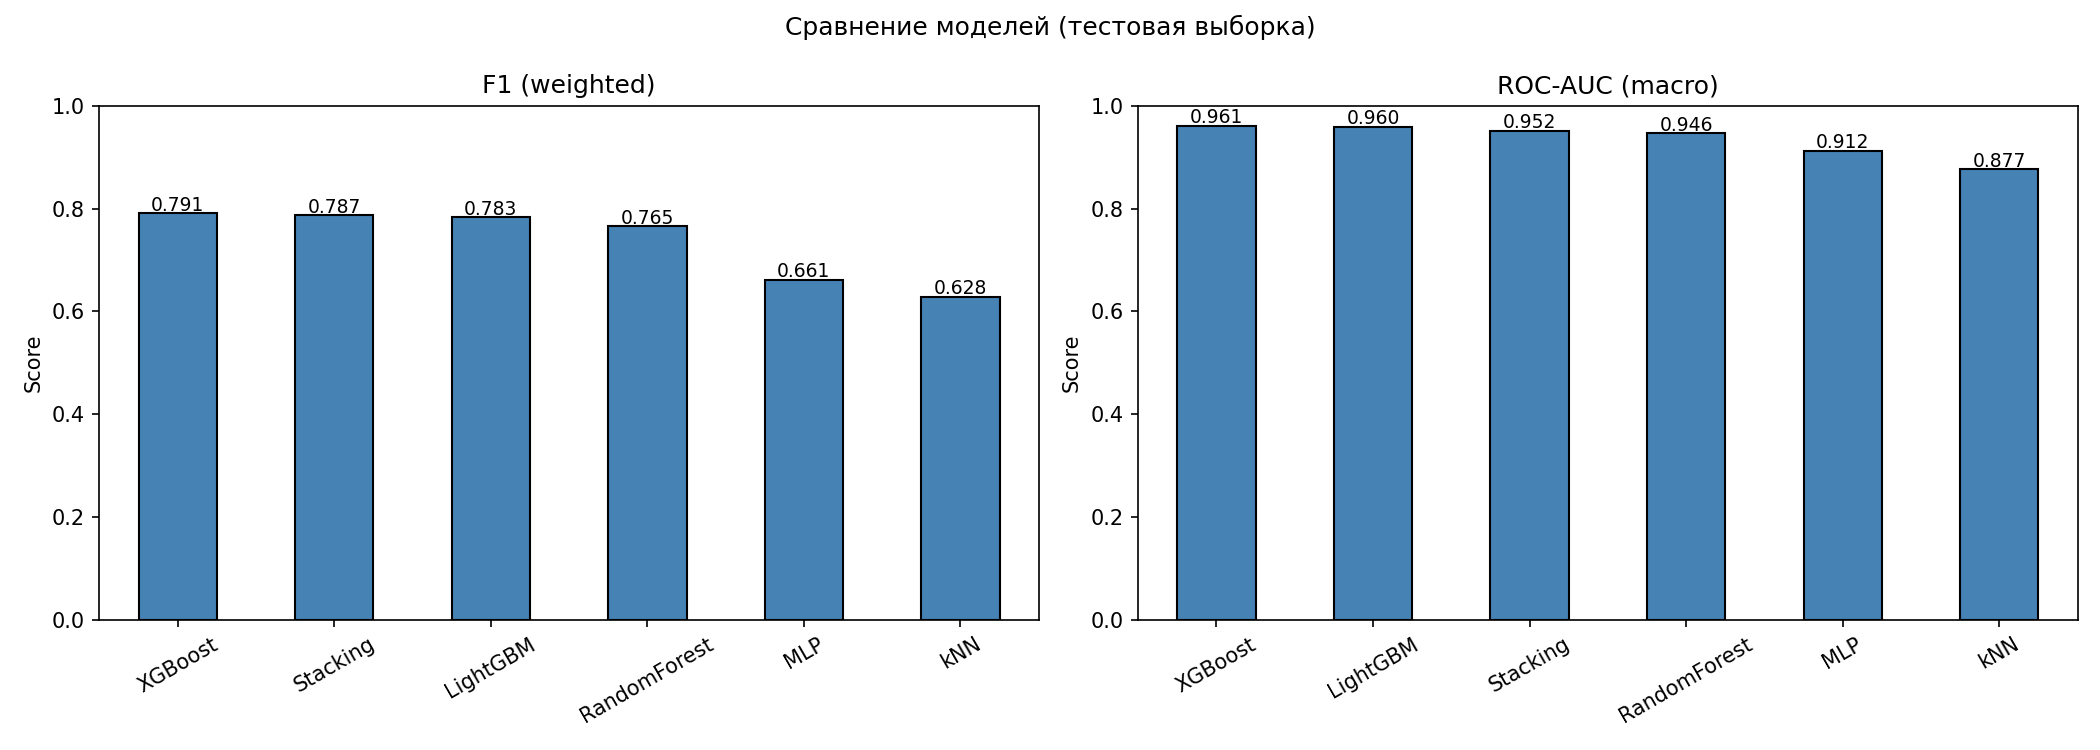
\includegraphics[width=\linewidth]{output/model_comparison.png}
    \caption{Сравнение всех моделей по взвешенной F1-мере~(слева) и макро-усреднённому ROC-AUC~(справа) на тестовой выборке}
    \label{fig:model_comparison}
\end{figure}

\subsection{Матрицы ошибок}

Матрица ошибок нормализована по строкам~--- элемент $M_{ij} = P(\hat{y}=j \mid y=i)$ показывает, с какой вероятностью объект истинного класса~$i$ предсказывается как класс~$j$. Диагональные элементы~$M_{ii}$ равны полноте~(recall) для каждого класса. Цвет ячейки кодирует значение вероятности: более тёмный оттенок соответствует большему значению. Идеальный классификатор имеет единицы на диагонали и нули вне неё; у реального~--- часть вероятностной массы смещена в недиагональные ячейки, отражая ошибки классификации. На рисунках~\ref{fig:cm_xgboost}--\ref{fig:cm_knn} представлены нормализованные матрицы ошибок для всех шести моделей.

\begin{figure}
    \centering
    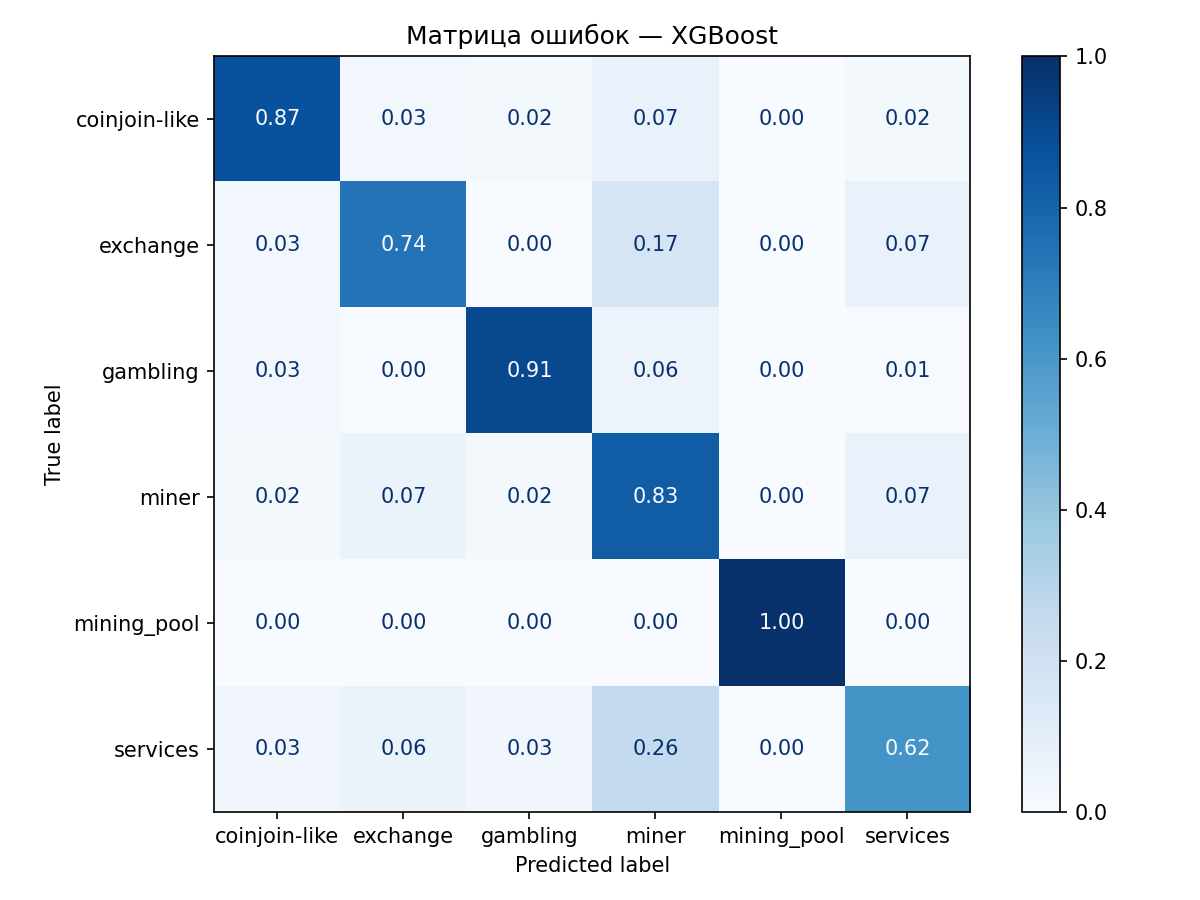
\includegraphics[width=0.82\linewidth]{output/confusion_matrix_XGBoost.png}
    \caption{Нормализованная матрица ошибок модели XGBoost на тестовой выборке}
    \label{fig:cm_xgboost}
\end{figure}

\begin{figure}
    \centering
    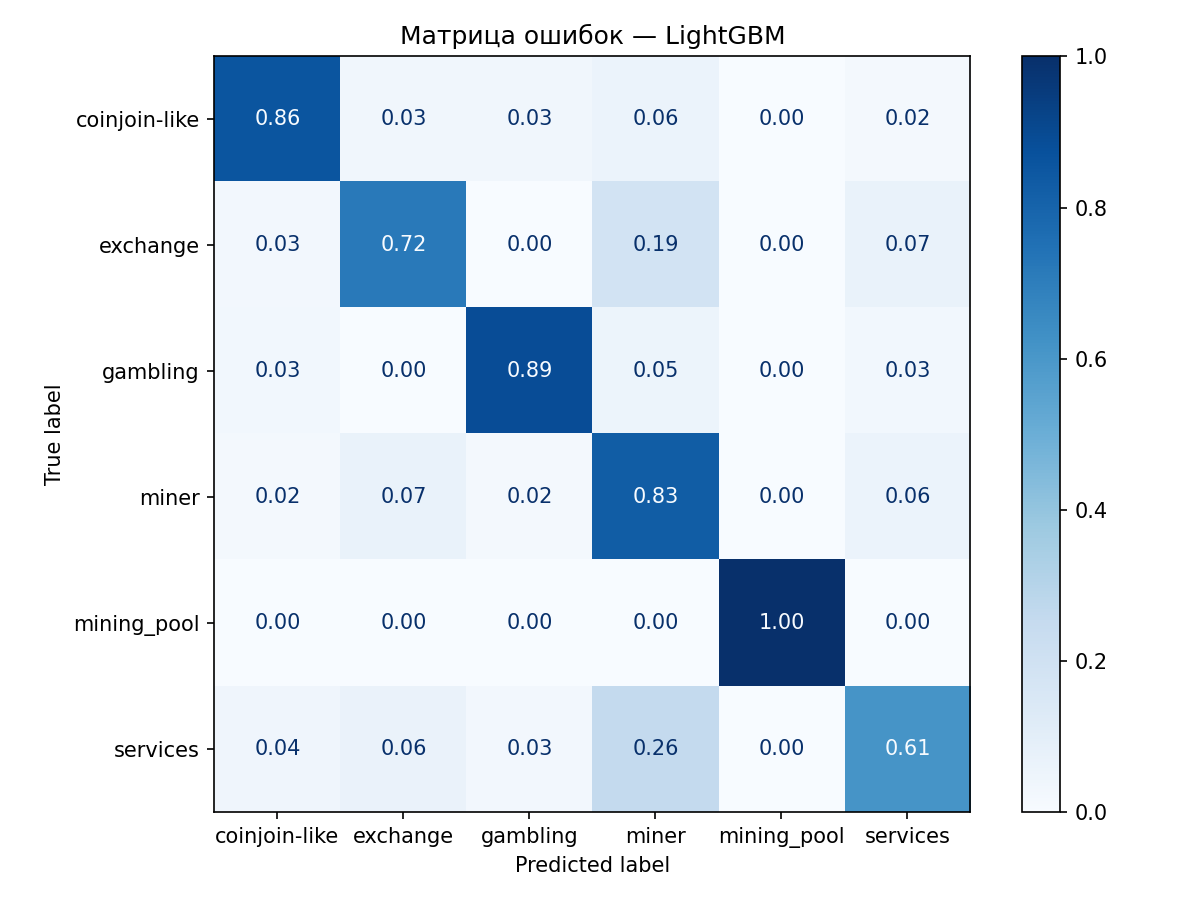
\includegraphics[width=0.82\linewidth]{output/confusion_matrix_LightGBM.png}
    \caption{Нормализованная матрица ошибок модели LightGBM на тестовой выборке}
    \label{fig:cm_lightgbm}
\end{figure}

\begin{figure}
    \centering
    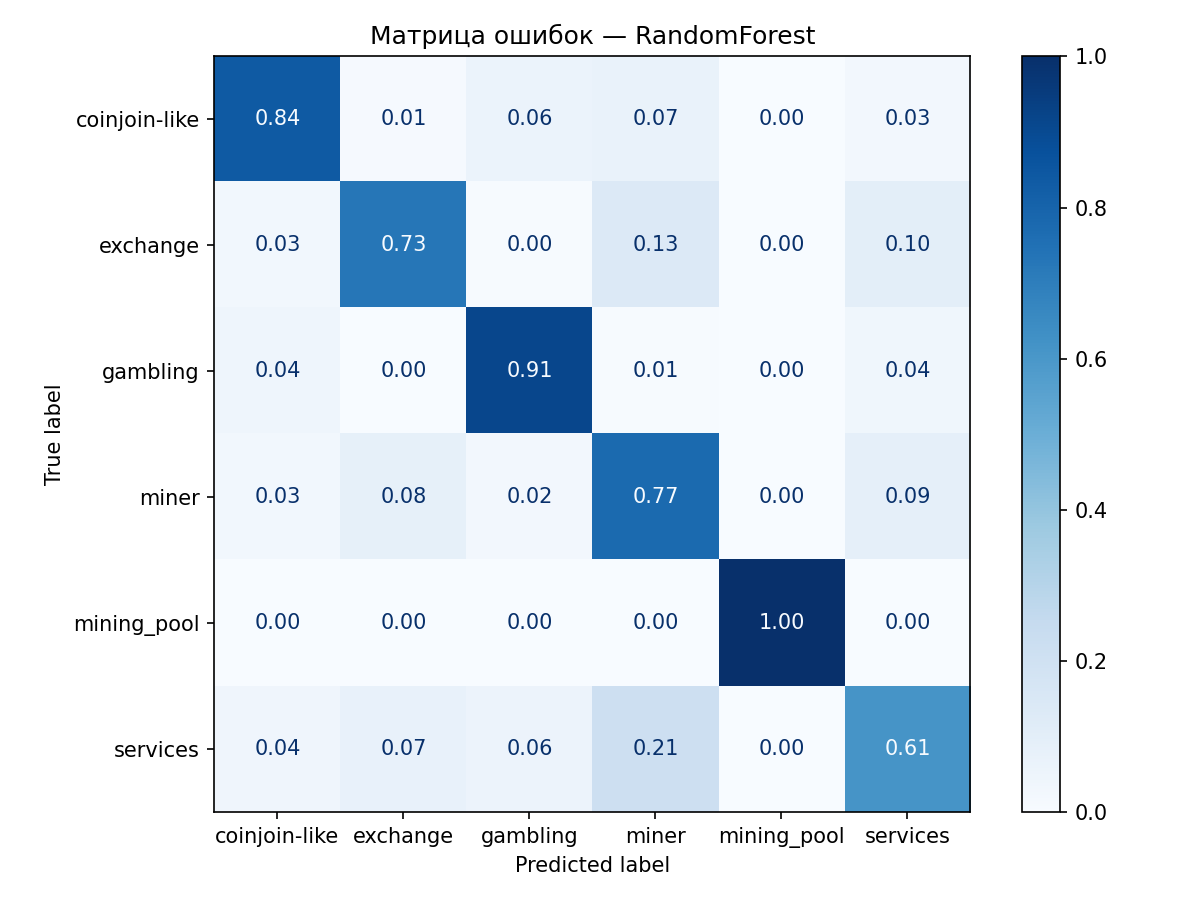
\includegraphics[width=0.82\linewidth]{output/confusion_matrix_RandomForest.png}
    \caption{Нормализованная матрица ошибок модели Random Forest на тестовой выборке}
    \label{fig:cm_rf}
\end{figure}

\begin{figure}
    \centering
    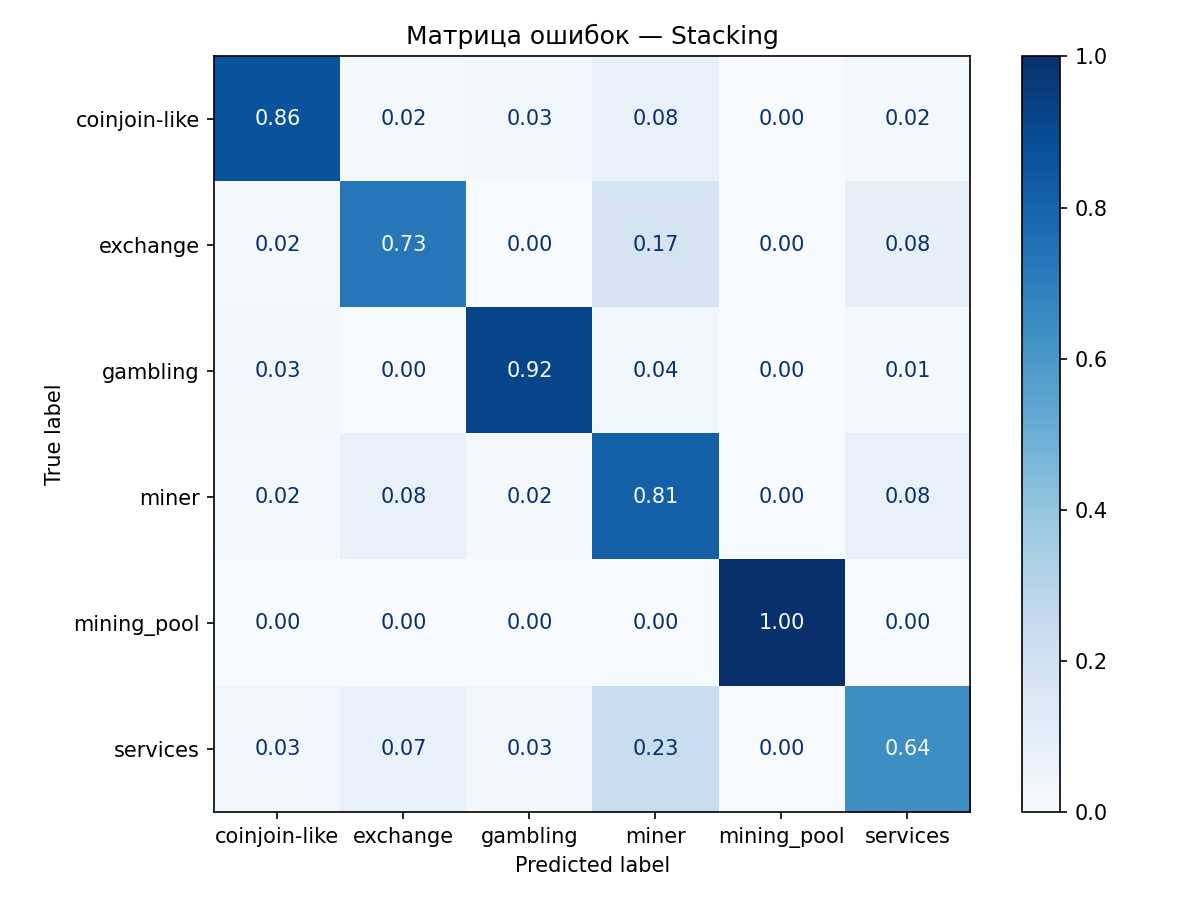
\includegraphics[width=0.82\linewidth]{output/confusion_matrix_Stacking.png}
    \caption{Нормализованная матрица ошибок модели Stacking на тестовой выборке}
    \label{fig:cm_stacking}
\end{figure}

\begin{figure}
    \centering
    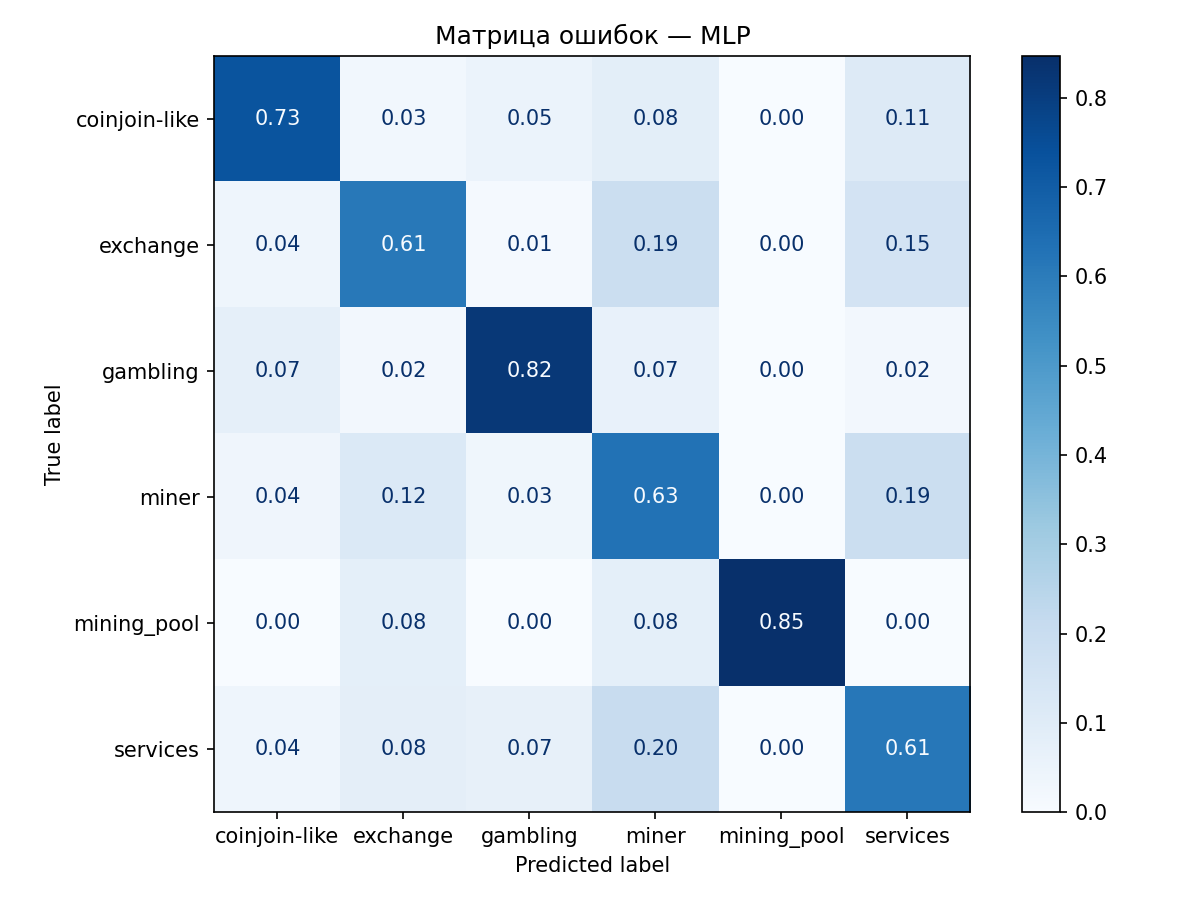
\includegraphics[width=0.82\linewidth]{output/confusion_matrix_MLP.png}
    \caption{Нормализованная матрица ошибок модели MLP на тестовой выборке}
    \label{fig:cm_mlp}
\end{figure}

\begin{figure}
    \centering
    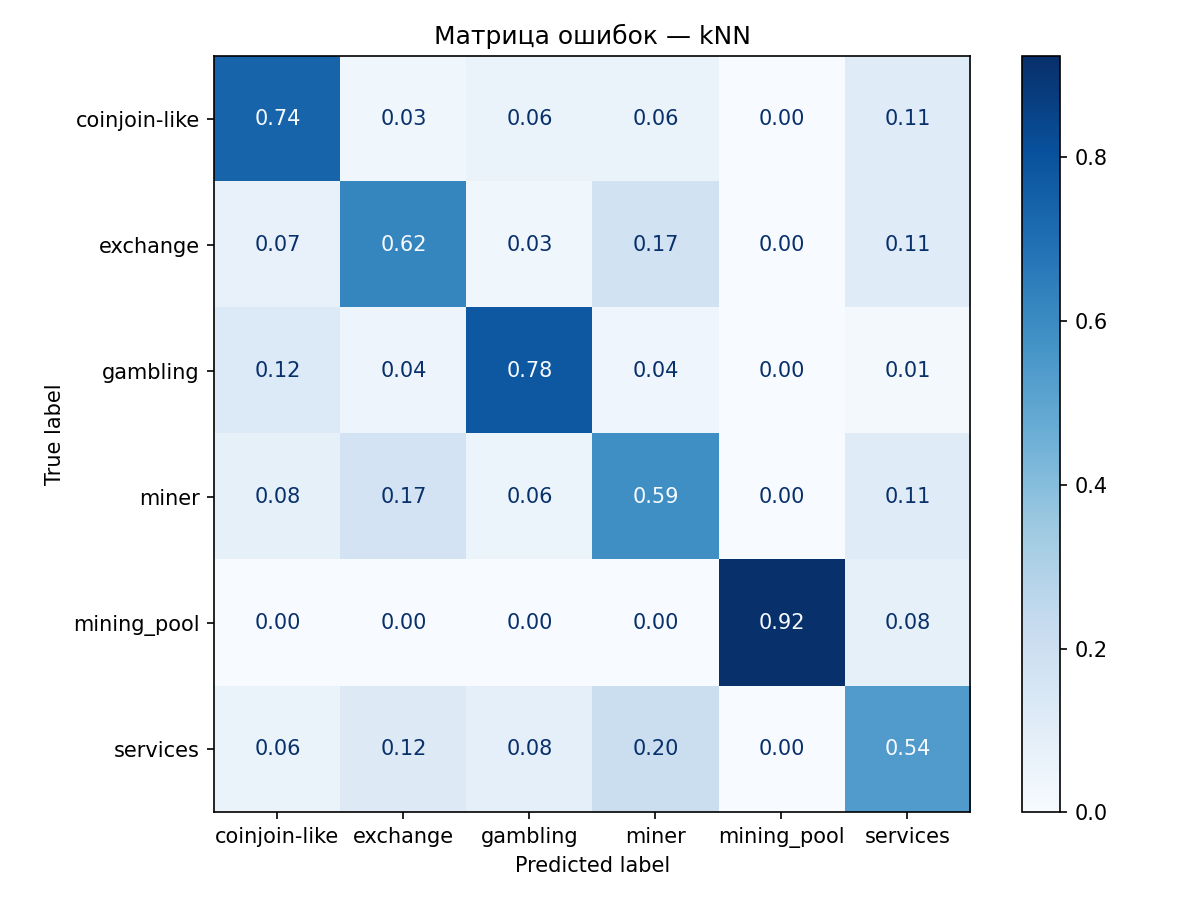
\includegraphics[width=0.82\linewidth]{output/confusion_matrix_kNN.png}
    \caption{Нормализованная матрица ошибок модели kNN на тестовой выборке}
    \label{fig:cm_knn}
\end{figure}

Анализ матриц ошибок~(рисунки~\ref{fig:cm_xgboost}--\ref{fig:cm_knn}) выявляет следующие закономерности. Наибольшую полноту у деревьевидных ансамблей показывают \textit{gambling}~(0,91) и \textit{coinjoin-like}~(0,87) как классы с наиболее характерными транзакционными паттернами; \textit{miner}~(0,83) и \textit{exchange}~(0,74) имеют умеренную полноту несмотря на бо́льшее представление в выборке. Класс \textit{services} устойчиво смешивается с \textit{miner}~--- 20--26\% объектов ошибочно классифицируются как \textit{miner} во всех моделях; у LightGBM~(рисунок~\ref{fig:cm_lightgbm}) доля таких ошибок составляет~26\%, у Random Forest~(рисунок~\ref{fig:cm_rf})~---~21\%. У деревьевидных ансамблей~(рисунки~\ref{fig:cm_xgboost}--\ref{fig:cm_stacking}) \textit{mining\_pool} классифицируется безошибочно~(recall~=~1,00); у MLP~(рисунок~\ref{fig:cm_mlp}) и kNN~(рисунок~\ref{fig:cm_knn}) наблюдается незначительная путаница с \textit{exchange} и \textit{miner}~(по~0,08). Матрицы MLP и kNN значительно более размыты~--- ошибки рассеяны между несколькими классами, что типично для менее мощных классификаторов на небольших табличных данных.

\subsection{ROC-кривые и оптимизация порогов классификации}

\subsubsection{Анализ ROC-кривых}

ROC-кривые построены для каждой модели в постановке OvR~(рисунки~\ref{fig:roc_xgboost}--\ref{fig:roc_knn}). В постановке OvR для шести классов строится шесть независимых бинарных задач: объекты класса~$c$ считаются положительными, все остальные~--- отрицательными; порог решения варьируется от~0 до~1, формируя совокупность пар~$(\text{FPR}_c,\,\text{TPR}_c)$, которые образуют ROC-кривую класса~$c$. Каждая кривая соответствует одному классу: ось~X~--- FPR, ось~Y~--- TPR; в легенде указан AUC для данного класса. Диагональная пунктирная линия соответствует случайному классификатору~(AUC~=~0,5). Площадь под кривой~(AUC) для класса~$c$ численно равна вероятности того, что случайно выбранный объект класса~$c$ получит более высокую оценку принадлежности к~$c$, чем случайно выбранный объект другого класса~--- данная интерпретация делает метрику независимой от порога классификации. Высокий AUC при низкой взвешенной F1 свидетельствует о хорошей ранжирующей способности модели при неоптимальном пороге классификации~0,5; оптимизация порогов по критерию Юдена для лучшей модели рассмотрена в подразделе~2.4.2.

\begin{figure}
    \centering
    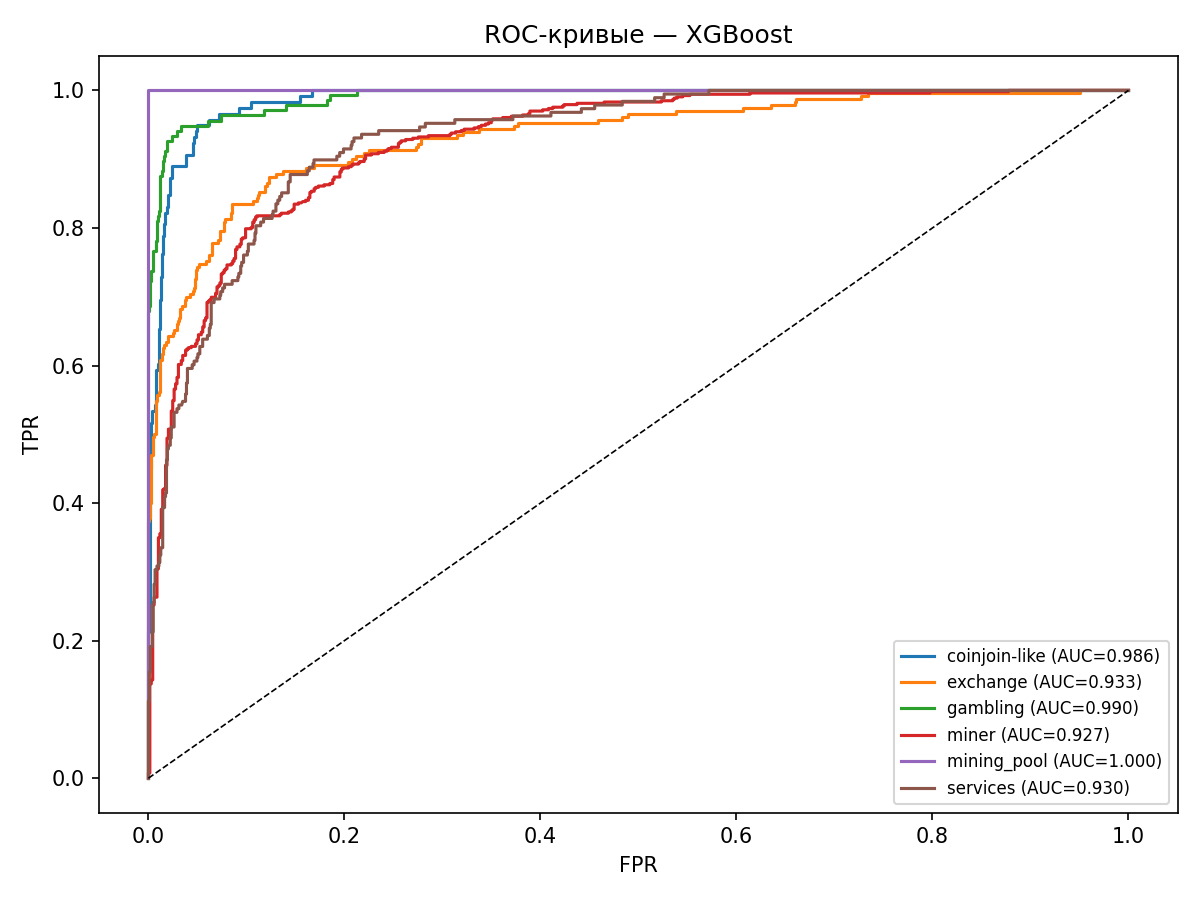
\includegraphics[width=0.82\linewidth]{output/roc_XGBoost.png}
    \caption{ROC-кривые в постановке OvR для модели XGBoost (макро ROC-AUC = 0,9610) на тестовой выборке}
    \label{fig:roc_xgboost}
\end{figure}

\begin{figure}
    \centering
    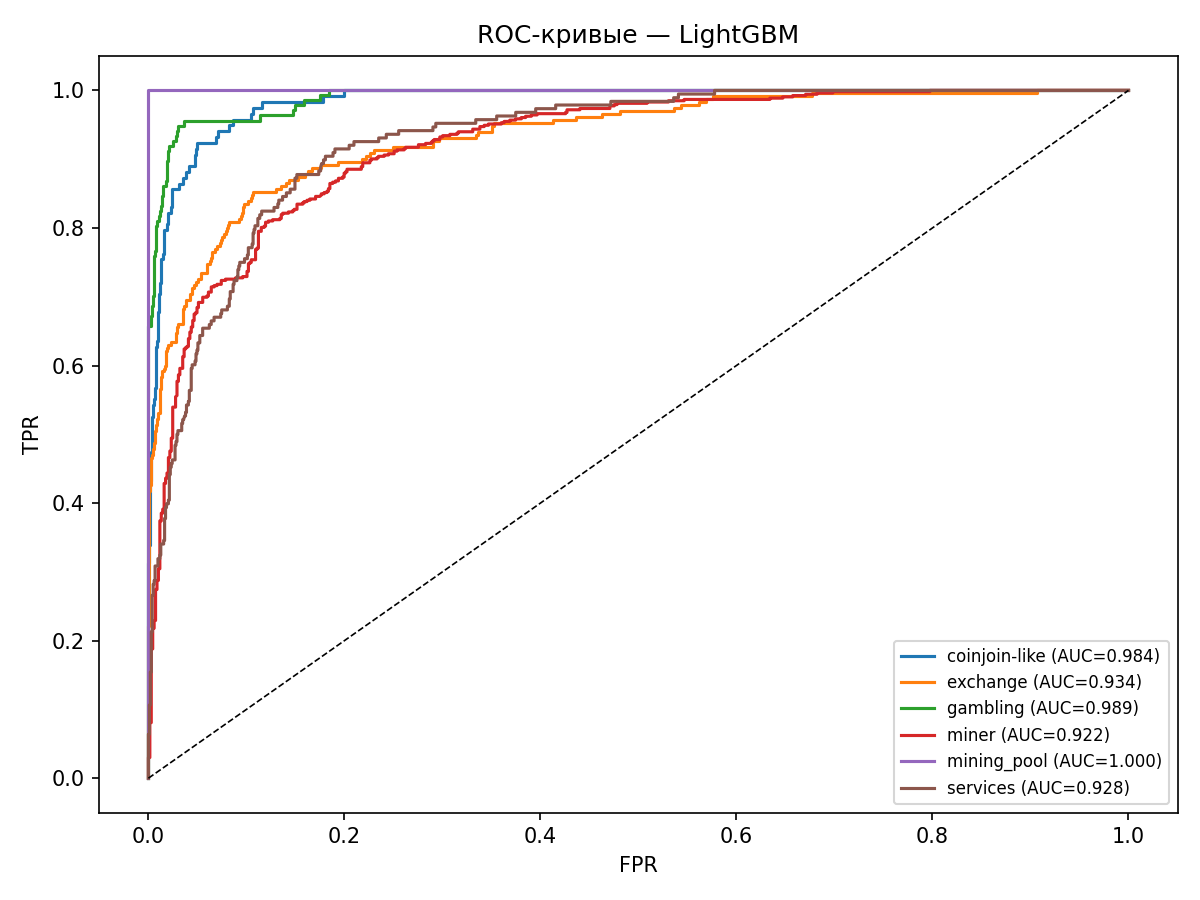
\includegraphics[width=0.82\linewidth]{output/roc_LightGBM.png}
    \caption{ROC-кривые в постановке OvR для модели LightGBM (макро ROC-AUC = 0,9597) на тестовой выборке}
    \label{fig:roc_lightgbm}
\end{figure}

\begin{figure}
    \centering
    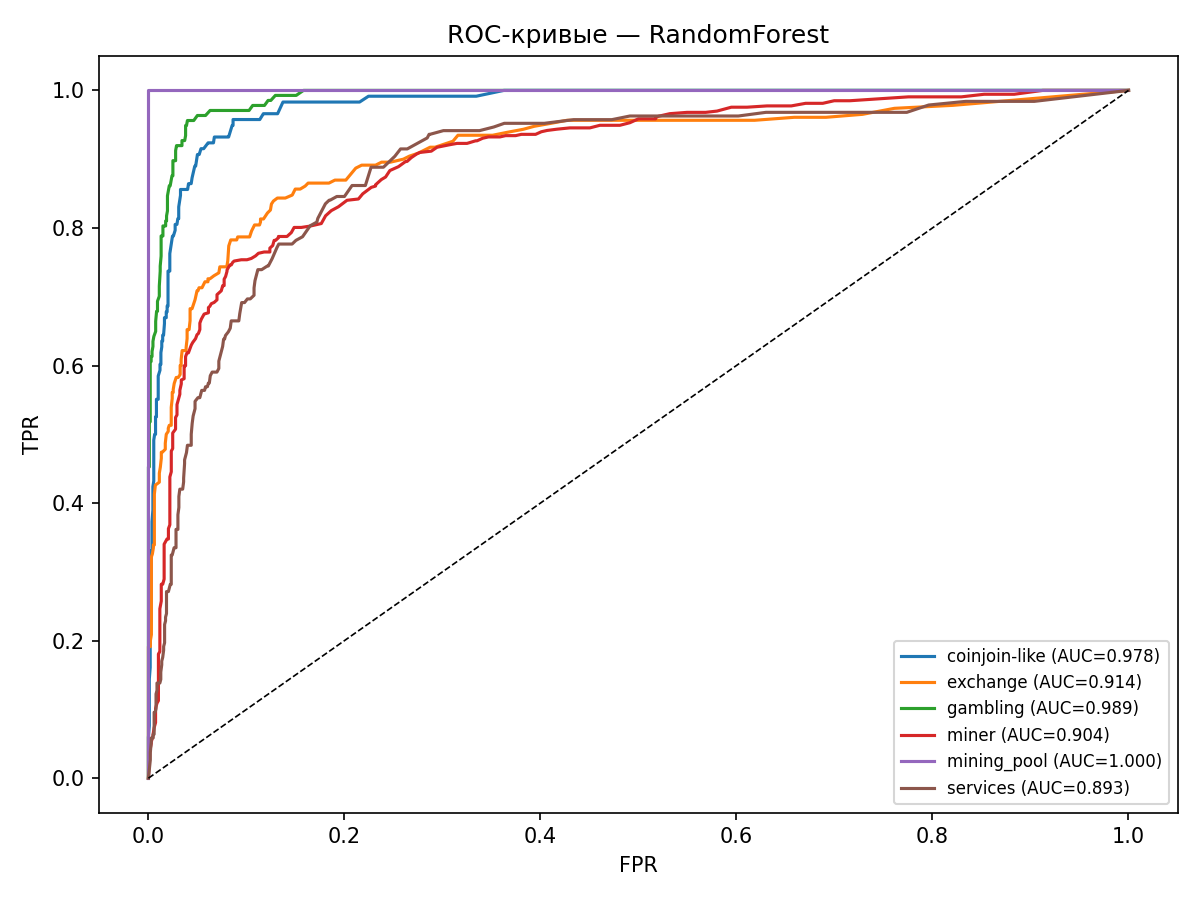
\includegraphics[width=0.82\linewidth]{output/roc_RandomForest.png}
    \caption{ROC-кривые в постановке OvR для Random Forest (макро ROC-AUC = 0,9463) на тестовой выборке}
    \label{fig:roc_rf}
\end{figure}

\begin{figure}
    \centering
    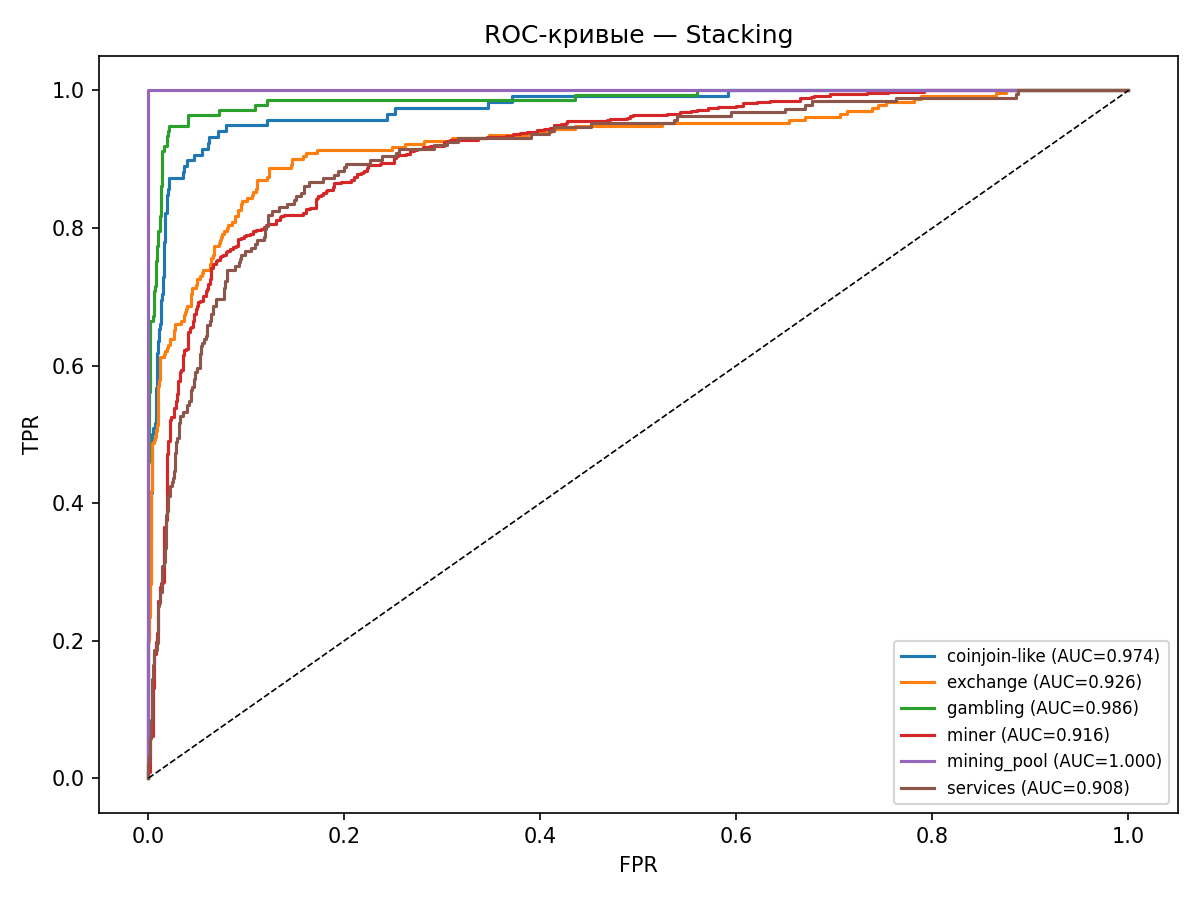
\includegraphics[width=0.82\linewidth]{output/roc_Stacking.png}
    \caption{ROC-кривые в постановке OvR для модели Stacking (макро ROC-AUC = 0,9517) на тестовой выборке}
    \label{fig:roc_stacking}
\end{figure}

\begin{figure}
    \centering
    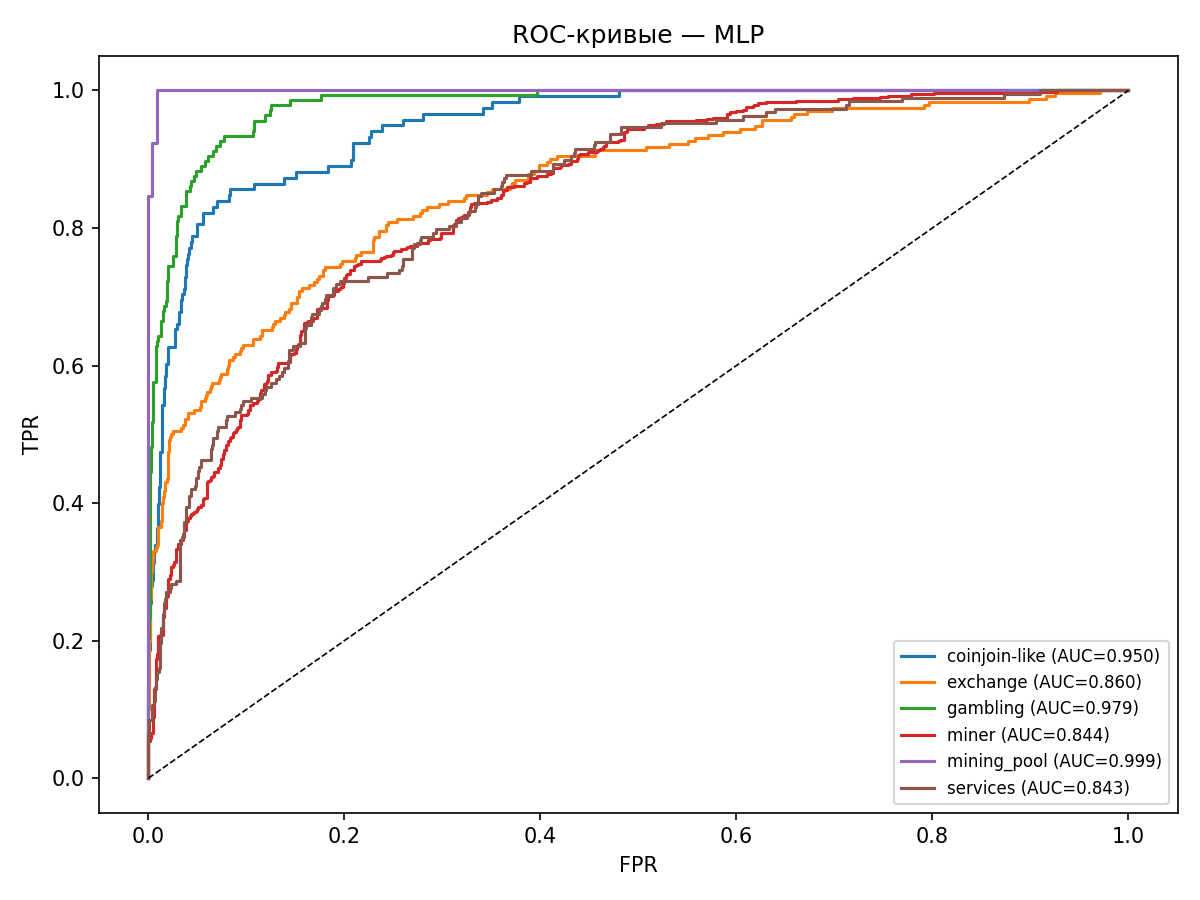
\includegraphics[width=0.82\linewidth]{output/roc_MLP.png}
    \caption{ROC-кривые в постановке OvR для модели MLP (макро ROC-AUC = 0,9124) на тестовой выборке}
    \label{fig:roc_mlp}
\end{figure}

\begin{figure}
    \centering
    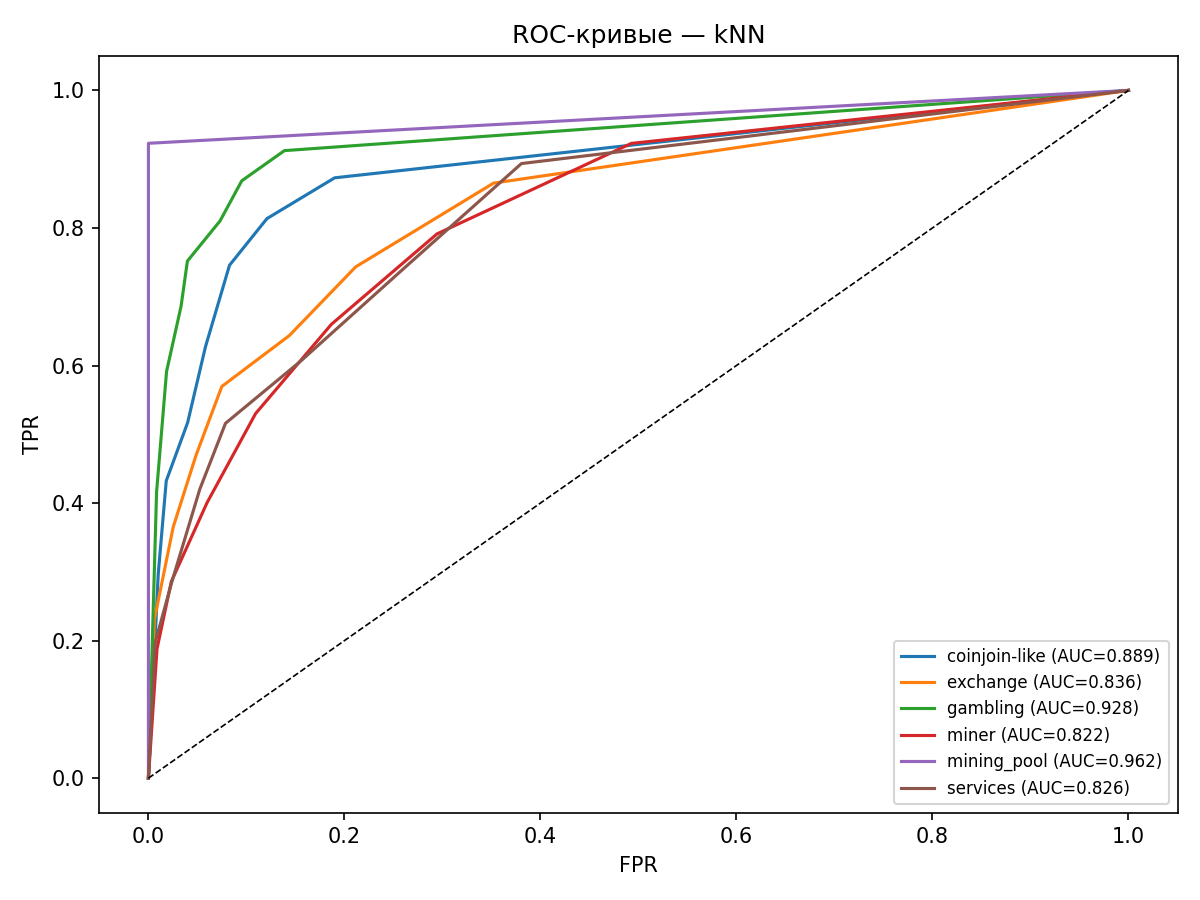
\includegraphics[width=0.82\linewidth]{output/roc_kNN.png}
    \caption{ROC-кривые в постановке OvR для модели kNN (макро ROC-AUC = 0,8769) на тестовой выборке}
    \label{fig:roc_knn}
\end{figure}

ROC-кривые XGBoost~(рисунок~\ref{fig:roc_xgboost}) и LightGBM~(рисунок~\ref{fig:roc_lightgbm}) демонстрируют крутой подъём в левой части: высокий TPR достигается при малом FPR, что отвечает требованиям~AML-систем. Stacking~(рисунок~\ref{fig:roc_stacking}) незначительно превосходит Random Forest~(рисунок~\ref{fig:roc_rf}) по AUC. Для MLP~(рисунок~\ref{fig:roc_mlp}) кривые ниже, чем у деревьевидных ансамблей, что отражает меньшую разделимость классов. Для kNN~(рисунок~\ref{fig:roc_knn}) кривые заметно ниже и менее упорядочены~--- метод не формирует хорошо калиброванных вероятностей в высокодимензиональном пространстве. Наименьший AUC во всех моделях~--- у класса~\textit{services}.

\subsubsection{Критерий Юдена и оптимизация порогов}

Для лучшей модели~(XGBoost) выполнена оптимизация порогов по критерию Юдена. Для класса~$c$ оптимальный порог определяется как $\tau_c^* = \arg\max_{\tau} J_c(\tau)$, где $J_c(\tau) = \text{TPR}_c(\tau) - \text{FPR}_c(\tau)$~--- статистика Юдена; $\text{TPR}_c(\tau)$~--- чувствительность (доля верно выявленных объектов класса~$c$) при пороге~$\tau$; $\text{FPR}_c(\tau)$~--- доля ложных тревог при пороге~$\tau$.
Итоговый класс: $\hat{y} = \arg\max_c (p_c(\mathbf{x}) - \tau_c^*)$. Оптимальные пороги оказываются ниже~0,5 для миноритарных классов~(\textit{mining\_pool},~\textit{coinjoin-like}), повышая их полноту. Взвешенная F1 при оптимизации~--- 0,7844~--- незначительно ниже исходных~0,7907: повышение полноты миноритарных классов сопровождается снижением точности мажоритарных, что незначительно снижает взвешенный агрегат, но важно для~AML-задач.

\subsection{Интерпретация предсказаний методом SHAP}

Метод~\acrshort{shap}~\cite{shap_paper} позволяет объяснить любое предсказание через значения Шепли из теории игр~--- справедливое распределение вклада каждого признака:
\begin{equation}\label{eq:shap}
    \phi_j = \sum_{S \subseteq \mathcal{F} \setminus \{j\}} \frac{|S|!\,(|\mathcal{F}|-|S|-1)!}{|\mathcal{F}|!}
    \bigl[f(\mathbf{x}_{S \cup \{j\}}) - f(\mathbf{x}_S)\bigr], \quad \sum_j \phi_j = f(\mathbf{x}) - \mathbb{E}[f],
\end{equation}
где $\phi_j$~--- значение Шепли признака~$j$, отражающее его вклад в конкретное предсказание, \\ $\mathcal{F}$~--- полное множество признаков, \\ $S \subseteq \mathcal{F} \setminus \{j\}$~--- подмножество признаков без~$j$, \\ $f(\mathbf{x}_{S \cup \{j\}})$~--- предсказание модели при наличии признаков из $S \cup \{j\}$, \\ $f(\mathbf{x}_S)$~--- предсказание без признака~$j$, \\ $\mathbb{E}[f]$~--- среднее предсказание по всей выборке.

Для XGBoost применён \textit{TreeExplainer}~--- точный полиномиальный алгоритм для ансамблей деревьев. Для MLP~--- \textit{PermutationExplainer} с~50~фоновыми образцами, использующий апроксимацию перестановками.

На рисунках~\ref{fig:shap_xgboost} и~\ref{fig:shap_mlp} представлены \textit{beeswarm}-диаграммы для XGBoost и MLP. Каждая точка~--- один объект тестовой выборки; горизонтальная ось~--- значение~SHAP (положительное сдвигает предсказание в сторону данного класса); цвет~--- исходное значение признака~(красный~--- высокое, синий~--- низкое).

\begin{figure}
    \centering
    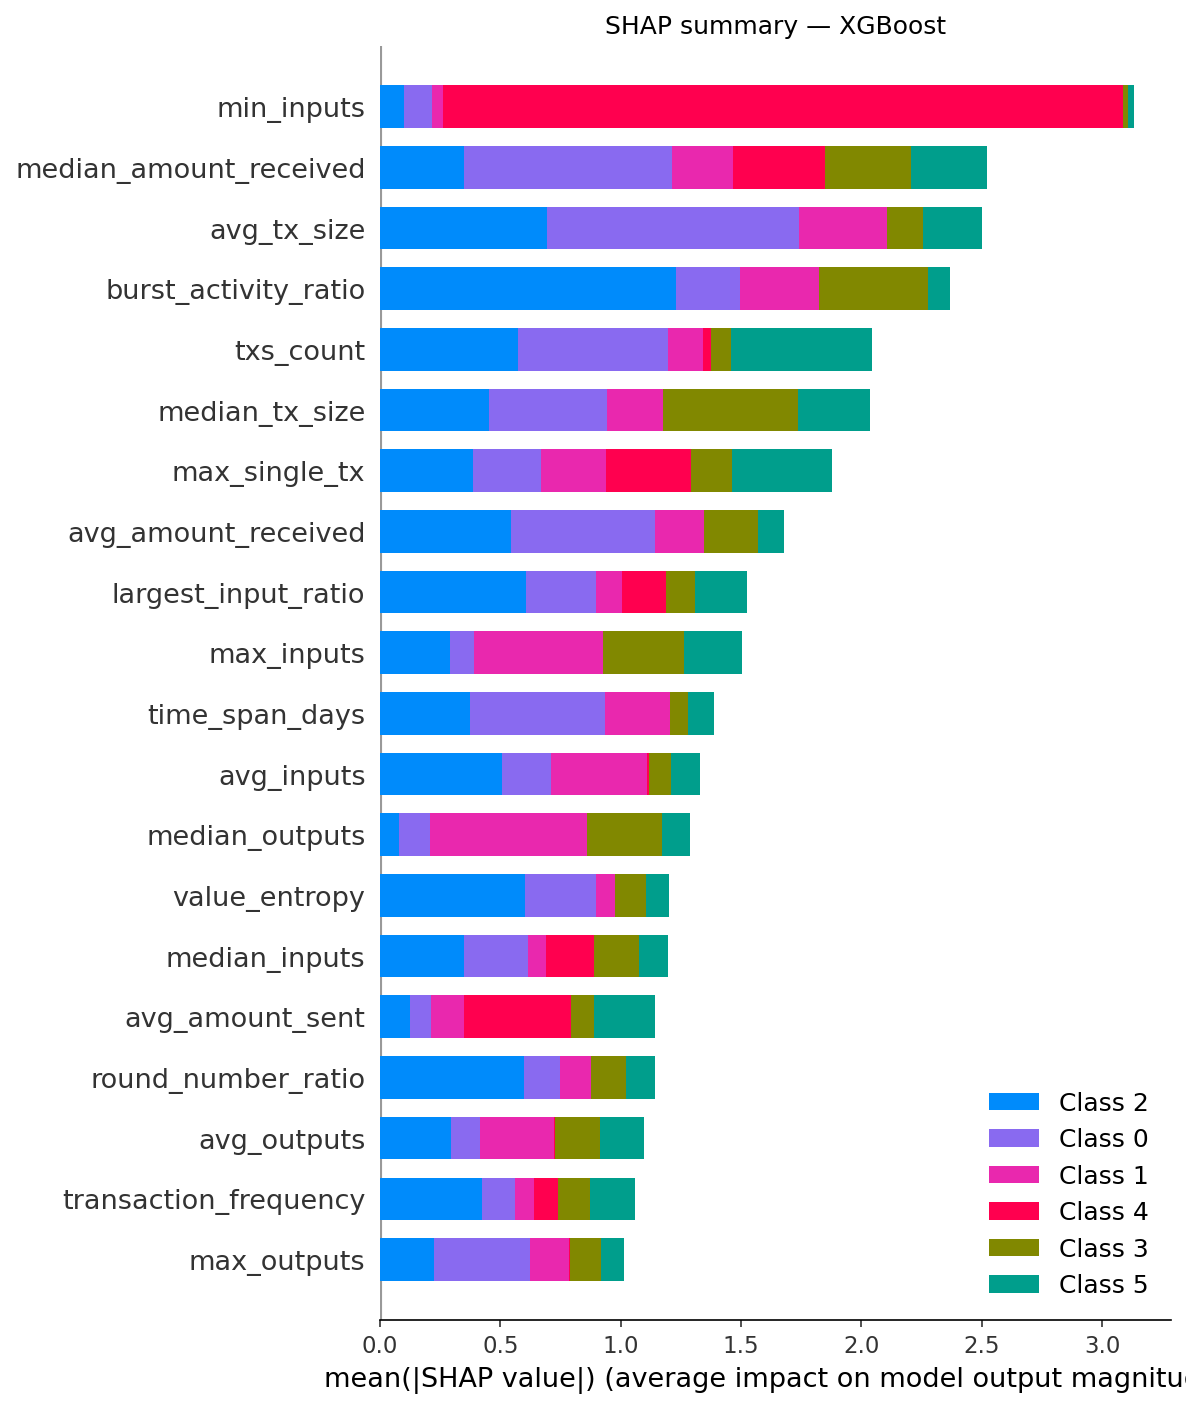
\includegraphics[width=\linewidth]{output/shap_summary_XGBoost.png}
    \caption{SHAP-диаграмма (\textit{beeswarm}) для модели XGBoost, построенная методом \textit{TreeExplainer}}
    \label{fig:shap_xgboost}
\end{figure}

\begin{figure}
    \centering
    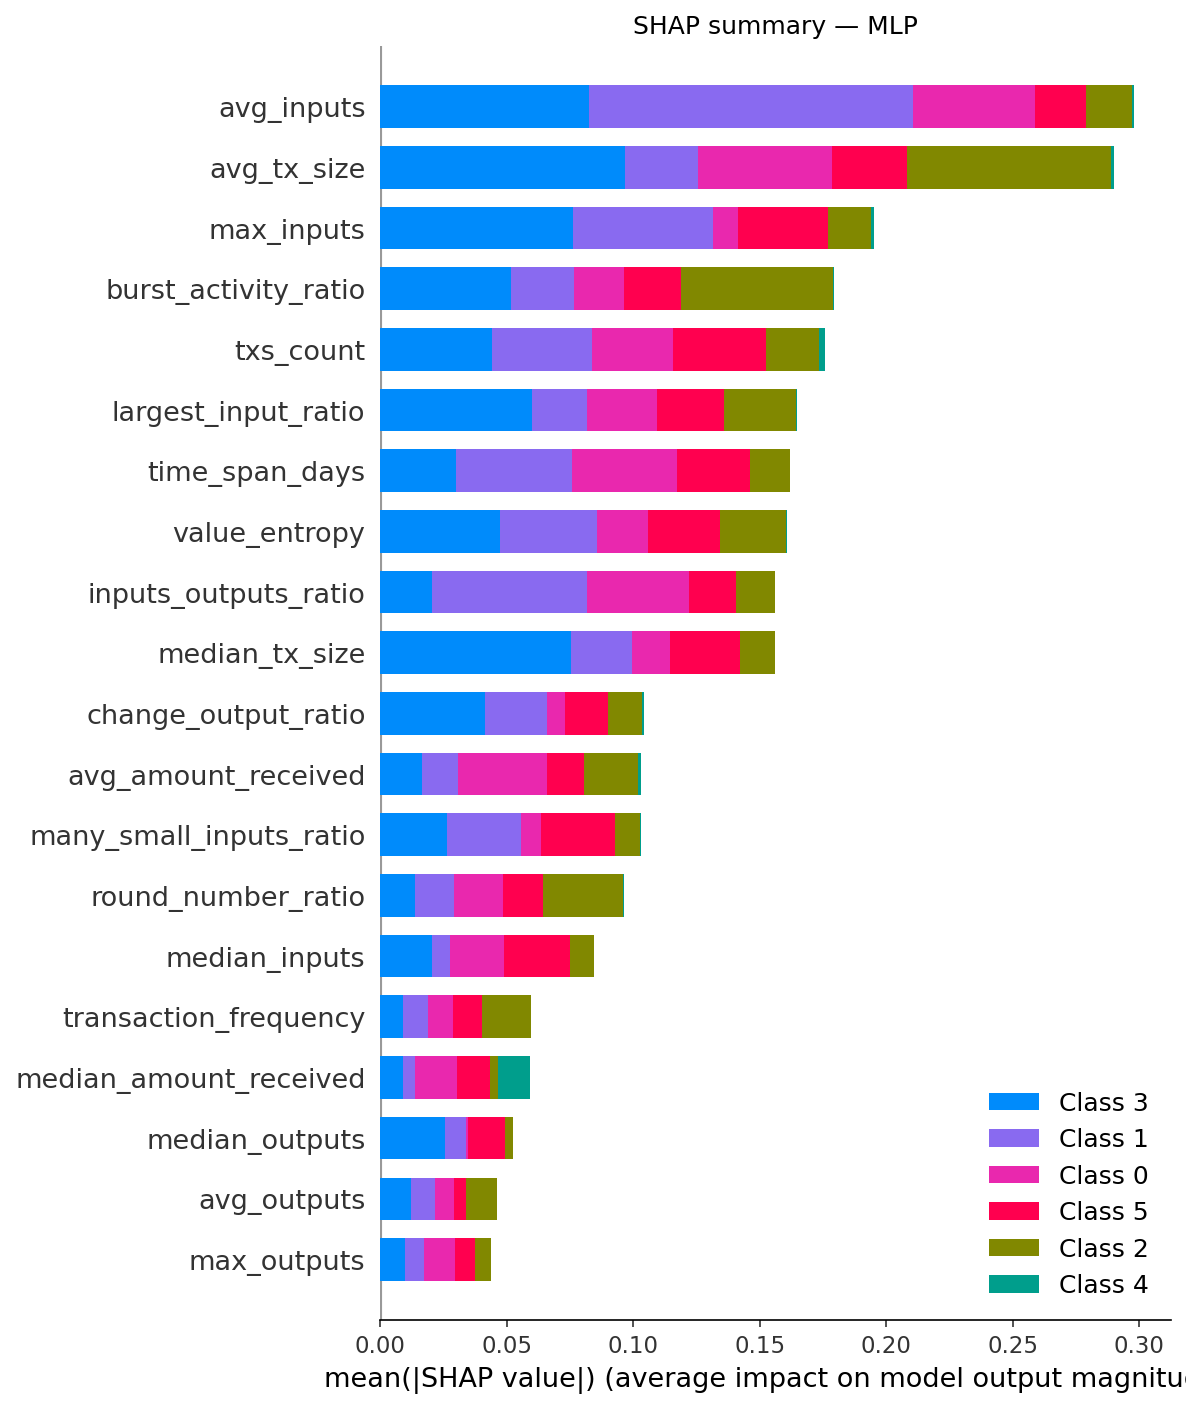
\includegraphics[width=\linewidth]{output/shap_summary_MLP.png}
    \caption{SHAP-диаграмма (\textit{beeswarm}) для модели MLP, построенная методом \textit{PermutationExplainer} с~50~фоновыми образцами}
    \label{fig:shap_mlp}
\end{figure}

По SHAP-диаграмме XGBoost~(рисунок~\ref{fig:shap_xgboost}) наибольший вклад вносят:
\begin{itemize}
    \item \textit{временны́е признаки}~--- среднее время между транзакциями и период активности: майнеры работают непрерывно с коротким ритмом, биржи~--- равномерно круглосуточно;
    \item \textit{экономические признаки}~--- средний объём и суммарный оборот: биржи обрабатывают на порядки больше, чем игровые адреса;
    \item \textit{структурные признаки}~--- число уникальных контрагентов, fan-out: пулы имеют много плательщиков, индивидуальные майнеры~--- мало;
    \item \textit{Bitcoin-специфичные}~--- SegWit, UTXO-паттерны: умеренный вклад, помогают идентифицировать~\textit{coinjoin-like}.
\end{itemize}

Рейтинг по SHAP совпадает с корреляционным анализом~НИРС-02 для топ-10 признаков~--- зависимости воспроизводимы. SHAP-диаграмма MLP~(рисунок~\ref{fig:shap_mlp}) показывает схожий порядок, однако значения распределены равномернее: XGBoost фокусируется на ключевых признаках точнее.

\subsection{Сравнительный анализ моделей}

Результаты подтверждают преимущество деревьевидных ансамблей над нейросетями на табличных данных~\cite{tabular_dl_survey}. Основные причины:
\begin{itemize}
    \item \textit{Явные условные зависимости}: деревья моделируют правила «если $x_j > t$ и $x_k < s$, то класс~$c$» напрямую; MLP аппроксимирует их через нелинейные комбинации весов, что требует больше параметров и данных.
    \item \textit{Инвариантность к распределению}: пороговые разбиения деревьев не зависят от формы распределения признаков; MLP чувствителен к скошенности даже после стандартизации.
    \item \textit{Объём данных}: 14\,892 образца недостаточно, чтобы реализовать потенциал MLP с архитектурой 256-128-64; регуляризация лишь частично компенсирует дефицит.
\end{itemize}

Stacking не превосходит XGBoost~--- базовые модели~(Random Forest, XGBoost и LightGBM) принадлежат одному классу методов и коррелируют в своих ошибках. Эффективнее было бы объединение XGBoost и MLP как принципиально разных подходов.

\subsection{Анализ проблемных классов}

Класс~\textit{services}~--- наиболее сложный: F1~$\approx$~0,65 у XGBoost, $\approx$~0,55 у MLP. Причины: неоднородный состав класса~(платёжные процессоры, миксеры, кошельковые сервисы); пересечение с~\textit{miner} по структурным признакам~--- в частности, по числу и минимальному размеру входов транзакций~(признак~\textit{min\_inputs} наиболее значим по SHAP); в тестовой выборке~187 объектов~--- оценка нестабильна. Рекомендации: детальная перемаркировка с разбиением на подкатегории, извлечение графовых признаков~(центральность, кластерный коэффициент), сбор дополнительных примеров.


    \conclusion
\begingroup\hyphenpenalty=10000\exhyphenpenalty=10000\sloppy
В рамках данной научно-исследовательской работы разработан и апробирован программный комплекс классификации Bitcoin-адресов по типу кошелька на основе датасета, сформированного в ходе НИРС-01 и НИРС-02. Реализован полный пайплайн подготовки данных: удаление коррелированных признаков, автоматический выбор стратегии устранения дисбаланса классов~(SMOTE превзошёл ADASYN по результатам прокси-сравнения на основе Random Forest) и стандартизация признаков. Обучено шесть моделей машинного обучения: MLP, Random Forest, XGBoost, LightGBM, Stacking и kNN. Для деревьевидных моделей произведена настройка гиперпараметров методом случайного поиска с двукратной стратифицированной кросс-валидацией. Проведена комплексная оценка качества: построены матрицы ошибок, ROC-кривые, вычислены взвешенная F1-мера и макро-усреднённый ROC-AUC для каждой модели. Сравнительный анализ показал явное преимущество деревьевидных методов над нейросетевой моделью на данной задаче: наилучший результат достигнут алгоритмом XGBoost~--- взвешенная F1-мера~0,7907, ROC-AUC~0,9610. Для лучшей модели выполнена оптимизация порогов классификации по критерию Юдена, повышающая полноту для миноритарных классов. Применение метода SHAP обеспечило интерпретируемость предсказаний и подтвердило значимость временны́х и экономических признаков. Детальный разбор ошибок выявил систематические паттерны смешения классов, прежде всего между \textit{services} и \textit{exchange}, и сформулированы гипотезы о путях улучшения. Практическая значимость работы определяется возможностью применения разработанного классификатора в системах AML-мониторинга криптовалютных операций, инструментах анализа блокчейн-активности и исследовательских задачах деанонимизации участников Bitcoin-сети. Результаты работы и исходный код доступны в открытом репозитории~\cite{github_repo_nirs3}. Перспективными направлениями дальнейших исследований являются: применение графовых нейронных сетей для учёта топологии транзакционного графа, расширение датасета и уточнение разметки класса~\textit{services}, разработка онлайн-системы обновления модели в условиях концептуального дрейфа, а также интеграция модели в реальную систему мониторинга.
\par\endgroup


\printbibliography

\end{document}
